% vim:filetype=tex ts=4 sw=4 noet foldmethod=indent foldmarker=\\begin,\\end foldcolumn=4 foldlevel=1 foldnestmax=1

\documentclass{beamer}
%\documentclass[handout]{beamer}

% For quick testing of a single frame:
%\includeonlyframes{current}

%\usetheme{CambridgeUS}

\usetheme{Dresden}
%\usetheme{Frankfurt}

% "Fixing" Dresden theme to look a bit like Frankfurt
\useoutertheme[subsection=false]{smoothbars}

%\usetheme{Copenhagen}
%\usetheme{Luebeck}
%\usetheme{Malmoe}
%\usetheme{Warsaw}

%\usecolortheme{dolphin}
\usecolortheme{whale}

% Useful small sizes: \scriptsize, \tiny, \Tiny, \TINY
\setbeamerfont{bibliography item}{size=\scriptsize}
\setbeamerfont{bibliography entry author}{size=\scriptsize}
\setbeamerfont{bibliography entry title}{size=\scriptsize}
\setbeamerfont{bibliography entry journal}{size=\scriptsize}
\setbeamerfont{bibliography entry location}{size=\scriptsize}
\setbeamerfont{bibliography entry note}{size=\scriptsize}

% Hiding navigation symbols
\setbeamertemplate{navigation symbols}{}


%%%%%%%%%%%%%%%%%%%%%%%%%%%%%%%%%%%%%%%%%%%%%%%%%%%%%%%%%%%%
% Font an encoding packages

% This does not accept all Unicode chars (for instance: I²C gives an error)
%\usepackage[utf8]{inputenc}

% This adds support for Unicode chars.
\usepackage{ucs}
\usepackage[utf8x]{inputenc}
% But should be avoided:
% http://tex.stackexchange.com/questions/13067/utf8x-vs-utf8-inputenc

\usepackage[brazil]{babel}

% http://tex.stackexchange.com/questions/664/why-should-i-use-usepackaget1fontenc
% http://texblog.net/latex-archive/fonts/symbols/
\usepackage[T1]{fontenc}


%%%%%%%%%%%%%%%%%%%%%%%%%%%%%%%%%%%%%%%%%%%%%%%%%%%%%%%%%%%%
% Embedding source-code

%\usepackage{color}
%\usepackage{xcolor}


% For inserting source-code
\usepackage{listings}

% Translating "Listing"
\renewcommand{\lstlistingname}{Listagem}

% Setting the default options
\lstset{
	basicstyle=\ttfamily\footnotesize,
	numberstyle=\scriptsize,
	numbers=left,
	escapeinside={(*@}{@*)},
	tabsize=4,
	breaklines=true,
	breakatwhitespace=true,
	showspaces=false,
	showstringspaces=false,
	showlines=false,
	captionpos=b
}
%	extendedchars=true,
%	inputencoding=utf8x,
%	numbersep=5pt,
%	frame=shadowbox,
%	frameround=rrrt,
%	rulecolor=\color{black},
%	rulesepcolor=\color{black},
% These don't seem to work if the caption is at the bottom
%	abovecaptionskip=\parskip,
%	belowcaptionskip=\parskip


% Dentro dos exemplos de código-fonte abaixo, coloquei um "tab" de
% indentação por estar dentro de um "frame", e "espaços" para a
% indentação do código de exemplo. Isto foi necessário porque os tabs
% estavam sendo ignorados dentro do códigos de exemplo.

\lstnewenvironment{ccodesmall}[1][]
{\lstset{language=C,
	basicstyle=\ttfamily\tiny,
	numberstyle=\tiny,
	#1}
}{}

\lstnewenvironment{ccode}[1][]
{\lstset{language=C,
	#1}
}{}

\lstnewenvironment{pythoncode}[1][]
{\lstset{language=Python,
	#1}
}{}

\lstnewenvironment{shellcode}[1][]
{\lstset{language=bash,
	#1}
}{}


%%%%%%%%%%%%%%%%%%%%%%%%%%%%%%%%%%%%%%%%%%%%%%%%%%%%%%%%%%%%
% Other packages

% 'microtype' improves LaTeX line-breaking algorithm by using
% microtypographic features of the font
% http://tex.stackexchange.com/questions/349/what-is-the-practical-difference-between-latex-and-pdflatex/358#358
\usepackage{microtype}

% http://en.wikibooks.org/wiki/LaTeX/Advanced_Mathematics
\usepackage{amsmath}
\DeclareMathOperator{\angulo}{ang}

% Adding \textsubscript{}
% LaTeX already has \textsuperscript, but lacks \textsubscript.
% http://en.wikibooks.org/wiki/LaTeX/Formatting#Text_mode_superscript_and_subscript
\usepackage{fixltx2e}

% Better handling of space after a custom command.
% http://tex.stackexchange.com/questions/17730/newcommand-and-spacing
\usepackage{xspace}

% 'booktabs' - Publication quality tables in LaTeX
\usepackage{booktabs}

% Required for including graphics
\usepackage{graphicx}

% http://tex.stackexchange.com/questions/10966/quickest-way-to-include-graphics/10972#10972
%\usepackage[rel]{overpic}

% Control the position of images/text in the slide/page:
% http://tex.stackexchange.com/questions/16357/how-can-i-position-an-image-in-an-arbitrary-position-in-beamer
% http://tex.stackexchange.com/questions/6817/insert-graphic-at-precise-place-on-a-page
% http://tex.stackexchange.com/questions/34921/how-to-overlap-images-in-a-beamer-slide
\usepackage{tikz}

% http://tex.stackexchange.com/questions/16189/repeat-command-n-times
\usepackage{pgffor}

% SI Units
% https://bitbucket.org/josephwright/siunitx/issue/100/undefined-control-sequence-bit-and-byte
\usepackage{siunitx}
\sisetup{
	load-configurations = binary,
	per-mode = symbol,
	list-final-separator = { e },
	range-phrase = { a },
	output-decimal-marker = {,}
}
\DeclareSIUnit\gauss{G}

% http://en.wikibooks.org/wiki/LaTeX/Formatting#Typesetting_URLs
\usepackage{hyperref}
\hypersetup{pdfborder={0 0 0}}


%%%%%%%%%%%%%%%%%%%%%%%%%%%%%%%%%%%%%%%%%%%%%%%%%%%%%%%%%%%%
% Custom commands
% http://tex.stackexchange.com/questions/1050/whats-the-difference-between-newcommand-and-newcommand

\newcommand*{\VBUS}{V\textsubscript{BUS}\xspace}
\newcommand*{\VCC}{V\textsubscript{CC}\xspace}
\newcommand*{\VDD}{V\textsubscript{DD}\xspace}


%%%%%%%%%%%%%%%%%%%%%%%%%%%%%%%%%%%%%%%%%%%%%%%%%%%%%%%%%%%%
% Other notes

% \linewidth is either \columnwidth in two-column mode or \textwidth in one-column mode.
% http://tex.stackexchange.com/questions/275/how-to-find-the-textwidth-in-two-column-mode/3531#3531


%%%%%%%%%%%%%%%%%%%%%%%%%%%%%%%%%%%%%%%%%%%%%%%%%%%%%%%%%%%%
% Some metadata

\title{Dispositivo apontador com interface USB usando magnetômetro}
\author{Denilson Figueiredo de Sá}
\date{2011-11-16}
\institute{DCC/UFRJ}
\keywords{AVR, USB, mouse, magnetometer}


% Shaded items in TOC will be 75% opaque
\setbeamertemplate{section in toc shaded}[default][75]

\AtBeginSection[]
{
	\begin{frame}<beamer>{Conteúdo}
		\begin{columns}[t]
			\column{.5\textwidth}
			\tableofcontents[currentsection, sections={-2}]
			\column{.5\textwidth}
			\tableofcontents[currentsection, sections={3-}]
		\end{columns}
	\end{frame}
}


\begin{document}


\begin{frame}
	\titlepage
\end{frame}


\section{Motivação}

\subsection{Motivação e inspiração}

\begin{frame}{Motivação}
	\begin{center}
		\pause
		\Large{Projeto Final de Curso é obrigatório}

		\pause
		\bigskip

		\Large{E eu quero me formar}
	\end{center}
\end{frame}


\begin{frame}{Motivação}
	Eu queria um projeto...
	\pause
	\begin{itemize}[<+->]
		\item Desafiador
		\item Divertido
		\item Útil
	\end{itemize}
\end{frame}


\begin{frame}{Inspiração}
	\pause
	\begin{center}
		% Marcin Wichary
		\href{http://www.youtube.com/watch?v=ttavBa4giPc\#t=2m46s}{Google I/O 2011: The Secrets of Google Pac-Man: A Game Show}
		\url{http://www.youtube.com/watch?v=ttavBa4giPc\#t=2m46s}
		\begin{tikzpicture}
			\onslide<+->{
				\node (imgtitle) {
\includegraphics[width=1\linewidth]{img/GoogleIO-title.jpg}};
			}
			\onslide<+->{
				\node (img1) at (imgtitle.north west) [anchor=north west, rotate=7.5, yshift=-0.1\linewidth, xshift=0.0\linewidth] {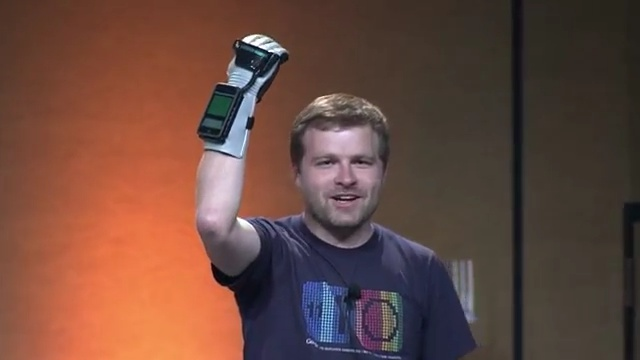
\includegraphics[width=0.5\linewidth]{img/GoogleIO-1.jpg}};
			}
			\onslide<+->{
				\node (img1) at (imgtitle.north east) [anchor=north east, rotate=-7.5, yshift=-0.1\linewidth, xshift=0.0\linewidth] {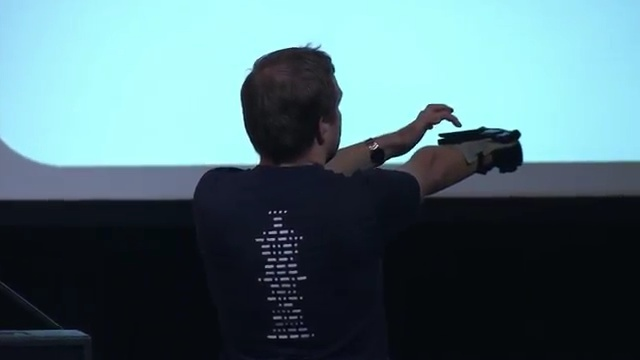
\includegraphics[width=0.5\linewidth]{img/GoogleIO-2.jpg}};
			}
			\onslide<+->{
				\node (img1) at (imgtitle.south) [anchor=south, rotate=0.0, yshift=0.0\linewidth, xshift=0.0\linewidth] {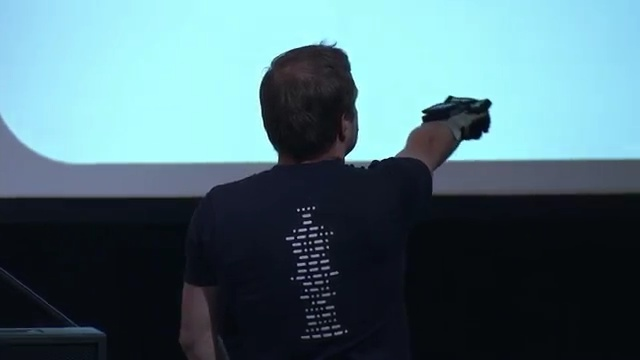
\includegraphics[width=0.5\linewidth]{img/GoogleIO-3.jpg}};
			}
		\end{tikzpicture}
	\end{center}
\end{frame}


\begin{frame}{É possível fazer menor}
	\begin{columns}
		\pause
		\column{.5\textwidth}
		\begin{center}
			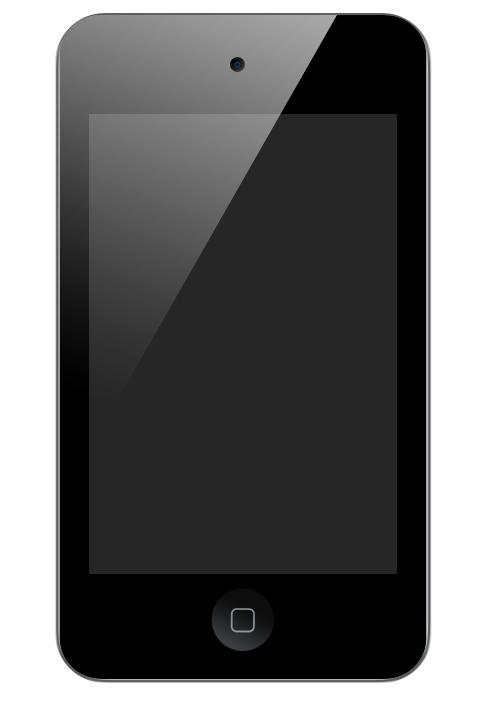
\includegraphics[width=0.8\textwidth]{img/IPod_touch_4G.png}

			\SI[product-units=single]{110 x 58 x 7}{\milli\metre}
		\end{center}

		\pause
		\column{.5\textwidth}
		\begin{center}
			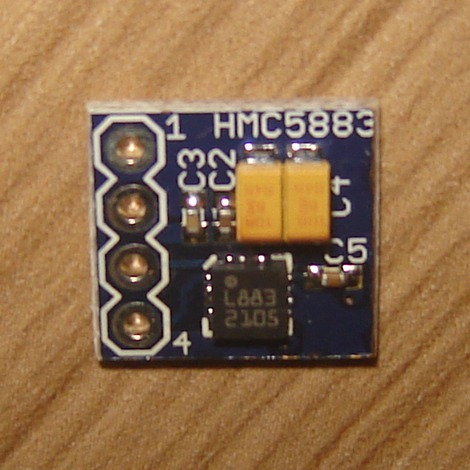
\includegraphics[width=0.19\textwidth]{../monografia/img/sensor_front.jpg}

			\SI[product-units=single]{11 x 11 x 4}{\milli\metre}
		\end{center}
	\end{columns}
\end{frame}


\begin{frame}{É possível fazer mais barato}
	\begin{columns}
		\pause
		\column{.5\textwidth}
		\begin{center}
			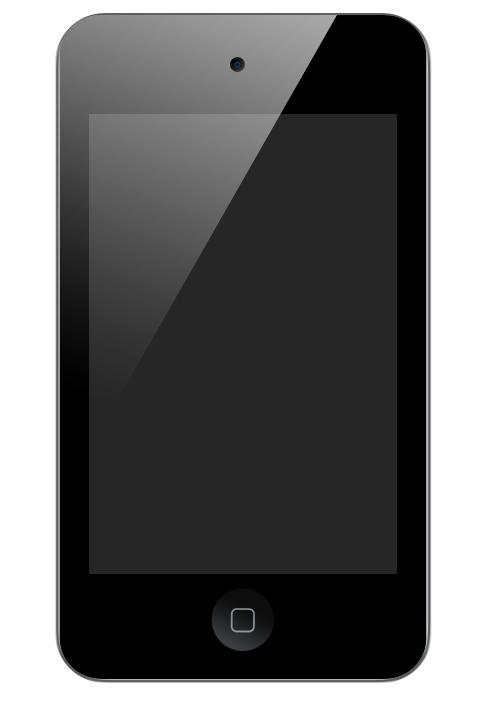
\includegraphics[width=0.8\textwidth]{img/IPod_touch_4G.png}

			R\$~729,00
		\end{center}

		\pause
		\column{.5\textwidth}
		\begin{center}
			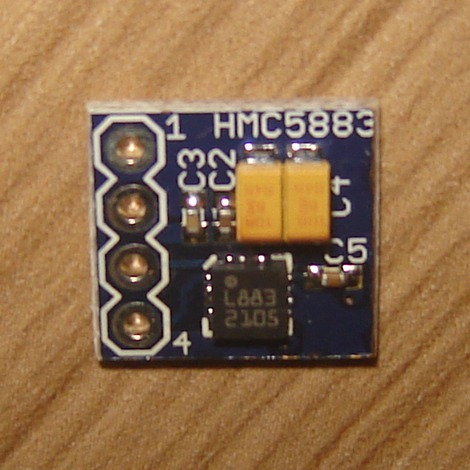
\includegraphics[width=0.19\textwidth]{../monografia/img/sensor_front.jpg}

			R\$~32,00

			\pause
			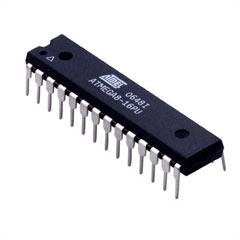
\includegraphics[width=0.35\textwidth]{img/ATmega8.jpg}

			R\$~10,00

			\pause
			\medskip

			Componentes diversos:

			R\$~20,00 a R\$~30,00

			\pause
			\medskip

			Preços de varejo!
		\end{center}
	\end{columns}
\end{frame}


\begin{frame}{É possível fazer mais compatível}
	\begin{center}
		\pause

		{\LARGE USB HID}

		\medskip

		Universal Serial Bus \\
		Human Interface Device

		\pause
		\bigskip

		Não requer instalação de drivers

		\medskip

		Plug-and-play
	\end{center}
\end{frame}


\section{Hardware}

\subsection{Microcontrolador}

\begin{frame}{ATmega8}
	\begin{columns}
		\column{.75\textwidth}
		\pause
		\begin{itemize}[<+->]
			\item Microcontrolador RISC de 8 bits
			\item Arquitetura Harvard, espaços distintos para instruções e variáveis
			\item 32 registradores de 8 bits de uso geral
			\item 1024 bytes de memória SRAM
			\item 512 bytes de memória EEPROM
			\item 8192 bytes de memória Flash \\
			equivalente a 4096 instruções
			\item \SI{12}{\mega\hertz} de clock, máximo de \SI{16}{\mega\hertz}
			\item Desempenho de até 1 instrução por ciclo
			\item Voltagem de \SIrange{4.5}{5.5}{\volt}
		\end{itemize}

		\column{.25\textwidth}
		\onslide<1->
		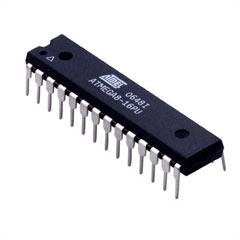
\includegraphics[width=1.0\textwidth]{img/ATmega8.jpg}
	\end{columns}
\end{frame}


\begin{frame}{Quão grande são \SI{8}{\kilo\byte}?}
	\begin{columns}
		\column{.5\textwidth}
		\pause
		\begin{center}
			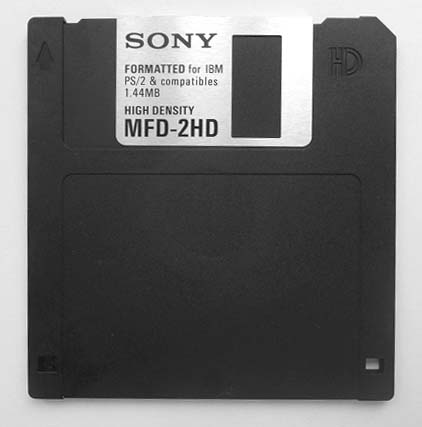
\includegraphics[width=1.0\textwidth]{img/floppy_disk.jpg}

			\SI{1440}{\kilo\byte}
		\end{center}

		\pause
		\column{.5\textwidth}
		\begin{center}
			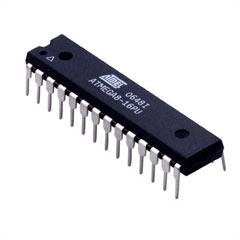
\includegraphics[width=0.0666666\textwidth]{img/ATmega8.jpg}
			\pause
			\foreach \n in {1,...,14} {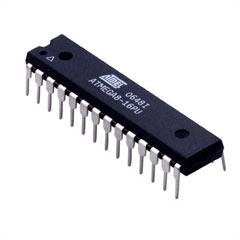
\includegraphics[width=0.0666666\textwidth]{img/ATmega8.jpg}}

			\foreach \m in {1,...,11} {
				\foreach \n in {1,...,15} {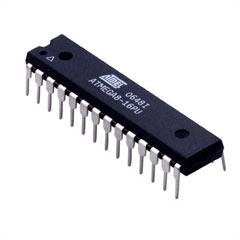
\includegraphics[width=0.0666666\textwidth]{img/ATmega8.jpg}}

			}

			\SI[parse-numbers = false]{180 \times 8}{\kilo\byte}
		\end{center}
	\end{columns}
\end{frame}


\subsection{Sensor}

\begin{frame}{HMC5883L}
	\begin{columns}
		\column{.75\textwidth}
		\pause
		\begin{itemize}[<+->]
			\item Magnetômetro, ou bússola eletrônica
			\item Intensidade do campo magnético em 3 eixos
			\item AMR - Anisotropic Magnetoresistance
			\item Precisão de \SIrange{1}{2}{\degree}
			\item ADC de 12 bits 
			\item Interface de comunicação I²C
			\item Medições a até \SI{75}{\hertz} ou \SI{160}{\hertz}
			\item Cada medição é uma média de 1, 2, 4 ou 8 leituras
			\item Voltagem de \SIrange{2.16}{3.6}{\volt}
		\end{itemize}

		\column{.25\textwidth}
		\onslide<1->
		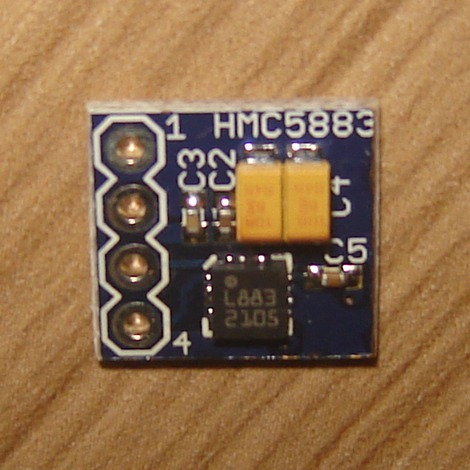
\includegraphics[width=1.0\textwidth]{../monografia/img/sensor_front.jpg}

		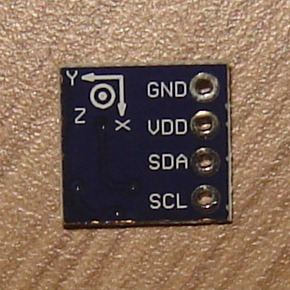
\includegraphics[width=1.0\textwidth]{../monografia/img/sensor_back.jpg}
	\end{columns}
\end{frame}


\begin{frame}[label=fotos-sensor]{HMC5883L}
	\begin{columns}
		\column{.5\textwidth}
		\begin{center}
			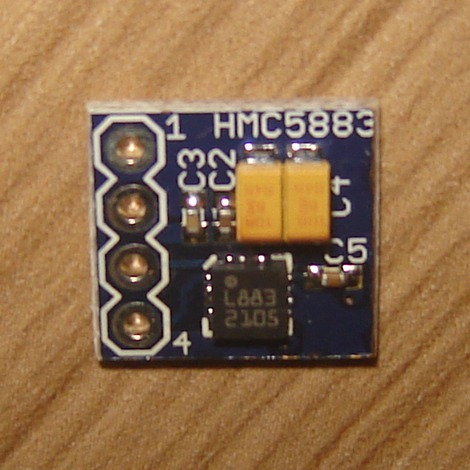
\includegraphics[height=0.4\textheight]{../monografia/img/sensor_front.jpg}

			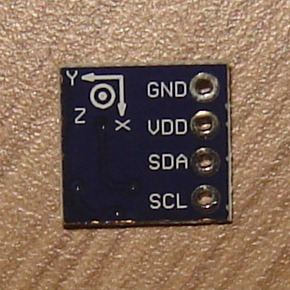
\includegraphics[height=0.4\textheight]{../monografia/img/sensor_back.jpg}
		\end{center}

		\column{.5\textwidth}
		\begin{center}
			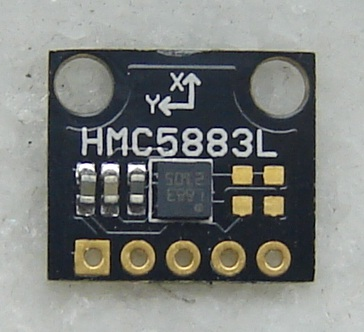
\includegraphics[height=0.4\textheight]{../monografia/img/sensor_other_pcb_front.jpg}

			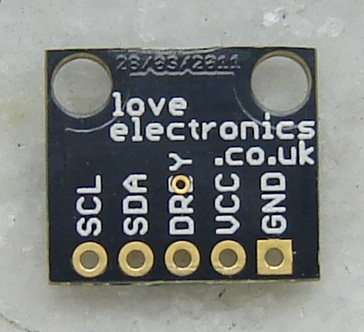
\includegraphics[height=0.4\textheight]{../monografia/img/sensor_other_pcb_back.jpg}
		\end{center}
	\end{columns}
\end{frame}


\subsection{Circuito}

\begin{frame}[plain, label=circuito-portrait]
%\begin{frame}[plain, label=circuito-portrait]{Diagrama do circuito}
	\begin{center}
		% 3.33 × 4.67 inch
		%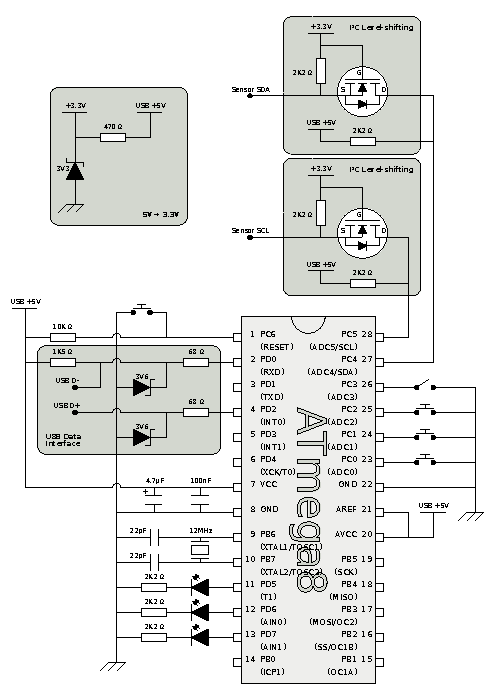
\includegraphics[keepaspectratio, width=1.0\textwidth, height=1.0\textheight]{../monografia/img/AVR-magnetometer-usb-mouse.pdf}
		% trim parameter order: left bottom right top
		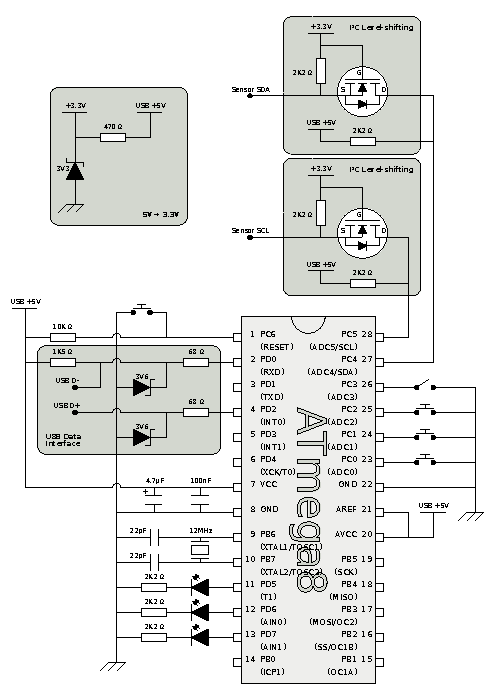
\includegraphics[keepaspectratio, width=1.0\textwidth, height=1.0\textheight, clip, trim=0.00in 0.10in 0.00in 0.10in]{../monografia/img/AVR-magnetometer-usb-mouse.pdf}
	\end{center}
\end{frame}

\begin{frame}[plain, label=circuito-landscape]
%\begin{frame}[plain, label=circuito-landscape]{Diagrama do circuito}
	\begin{center}
		%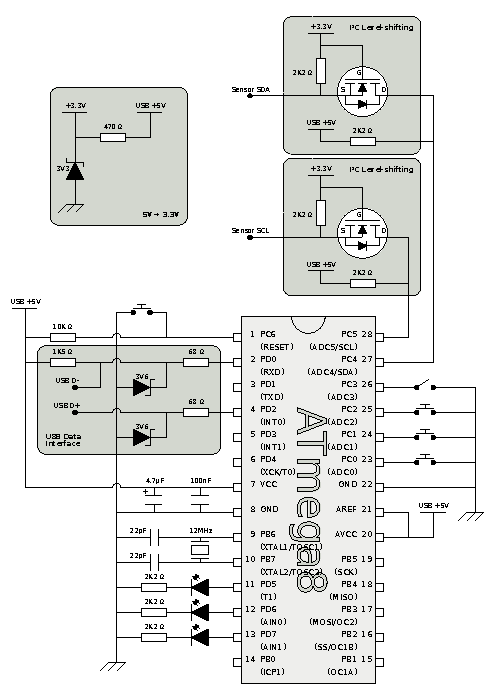
\includegraphics[angle=90, keepaspectratio, width=1.0\textwidth, height=1.0\textheight]{../monografia/img/AVR-magnetometer-usb-mouse.pdf}
		% trim parameter order: left bottom right top
		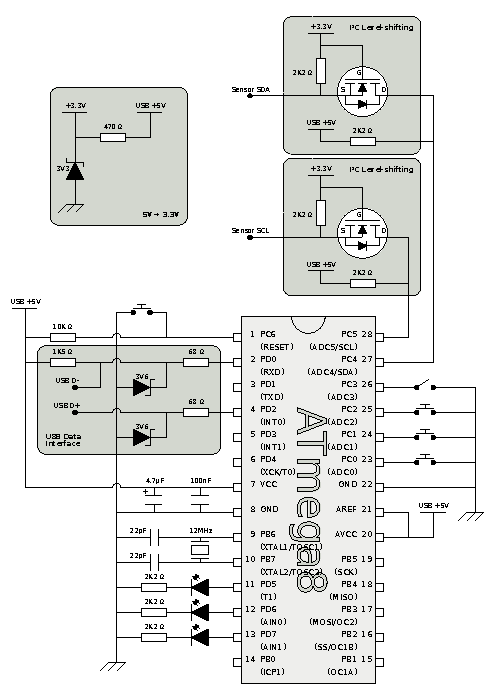
\includegraphics[angle=90, keepaspectratio, width=1.0\textwidth, height=1.0\textheight, clip, trim=0.00in 0.10in 0.00in 0.10in]{../monografia/img/AVR-magnetometer-usb-mouse.pdf}
	\end{center}
\end{frame}


\subsection{Interface USB}

\begin{frame}<1-4>[label=tensoes]{Tensões}
	\pause
	\begin{description}[<+->][HMC5883L]
		\item[USB \VBUS] \SIrange{4.4}{5.25}{\volt}
		\item[USB data]  \SIrange{2.8}{3.6}{\volt}
		\item[ATmega8]   \SIrange{4.5}{5.5}{\volt}
		\item[HMC5883L]  \SIrange{2.16}{3.6}{\volt}
	\end{description}
\end{frame}


\begin{frame}{Interface USB}
	\begin{center}
		% trim parameter order: left bottom right top
		%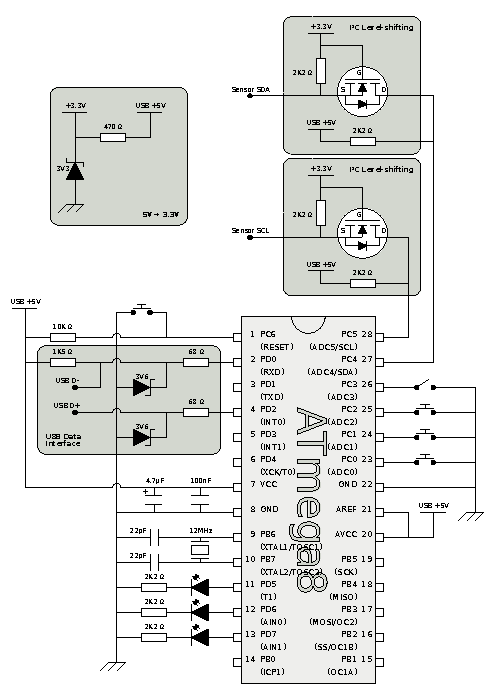
\includegraphics[keepaspectratio, width=1.0\textwidth, height=0.8\textheight, clip, trim=0.00in 1.20in 0.75in 2.00in]{../monografia/img/AVR-magnetometer-usb-mouse.pdf}
		% viewport parameter order: left bottom left+width bottom+height
		% Good size: width=3.3in height=2in
		%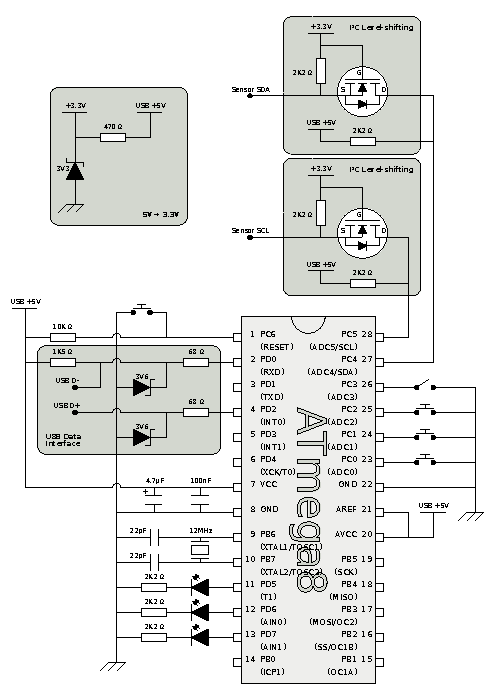
\includegraphics[keepaspectratio, width=1.0\textwidth, height=0.8\textheight, clip, viewport=0.00in 0.85in 2.66in 2.66in]{../monografia/img/AVR-magnetometer-usb-mouse.pdf}
		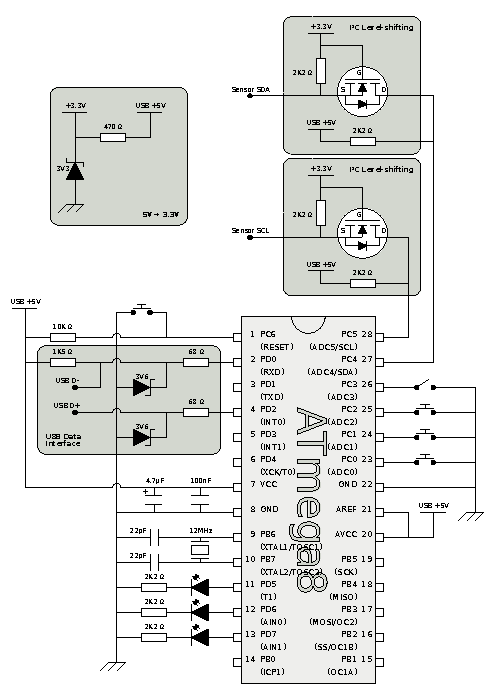
\includegraphics[keepaspectratio, width=1.0\textwidth, height=0.8\textheight, clip, viewport=0.00in 1.15in 2.66in 2.66in]{../monografia/img/AVR-magnetometer-usb-mouse.pdf}
	\end{center}
\end{frame}


\begin{frame}{Interface USB}
	\begin{center}
		% viewport parameter order: left bottom left+width bottom+height
		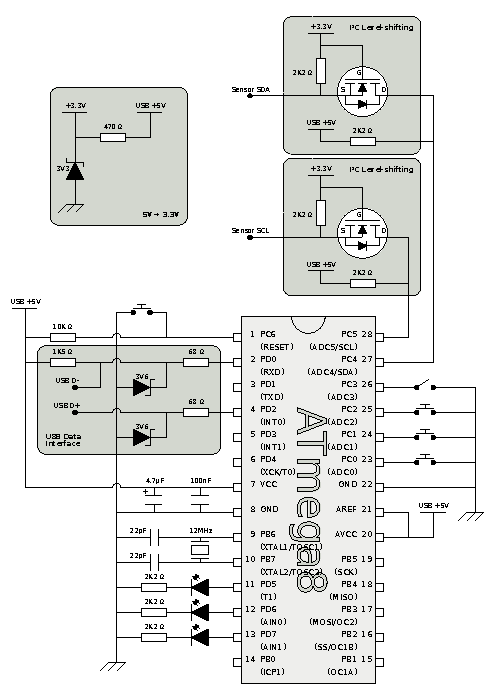
\includegraphics[keepaspectratio, width=1.0\textwidth, height=0.8\textheight, clip, viewport=0.00in 1.50in 2.00in 2.55in]{../monografia/img/AVR-magnetometer-usb-mouse.pdf}
	\end{center}
\end{frame}


\subsection{Interface com o sensor}

\againframe<4->{tensoes}


\begin{frame}{Interface com o sensor}
	\begin{center}
		% viewport parameter order: left bottom left+width bottom+height
		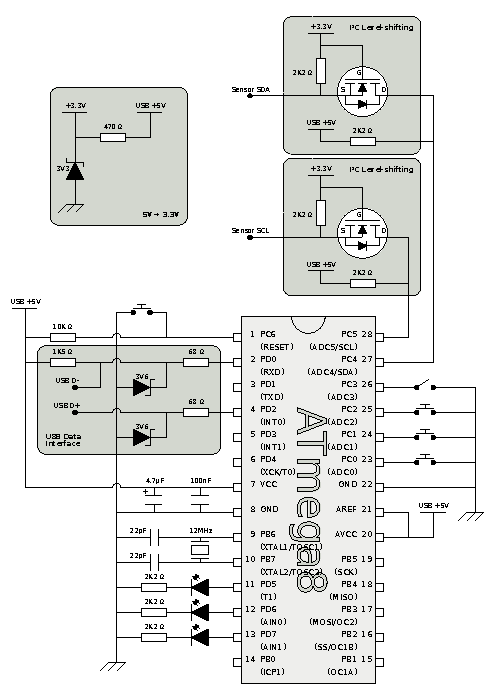
\includegraphics[keepaspectratio, width=1.0\textwidth, height=0.8\textheight, clip, viewport=0.00in 2.15in 3.33in 4.60in]{../monografia/img/AVR-magnetometer-usb-mouse.pdf}
	\end{center}
\end{frame}


\begin{frame}{Alimentação para o sensor}
	\begin{center}
		% viewport parameter order: left bottom left+width bottom+height
		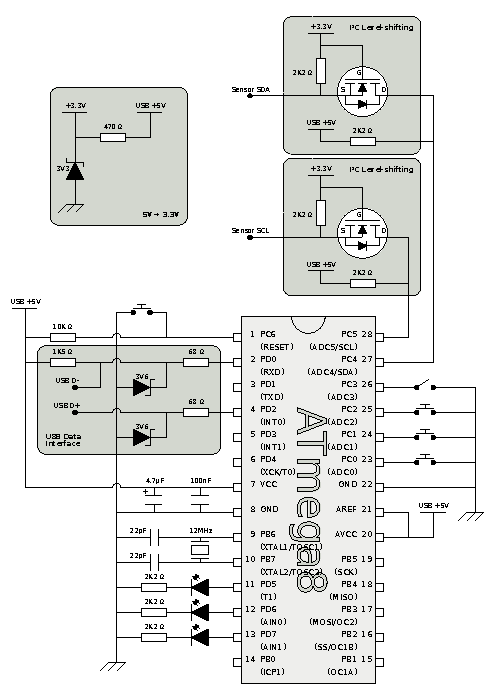
\includegraphics[keepaspectratio, width=1.0\textwidth, height=0.8\textheight, clip, viewport=0.00in 2.75in 1.80in 3.75in]{../monografia/img/AVR-magnetometer-usb-mouse.pdf}
	\end{center}
\end{frame}


\begin{frame}{I²C Level-shifting}
	\begin{center}
		% viewport parameter order: left bottom left+width bottom+height
		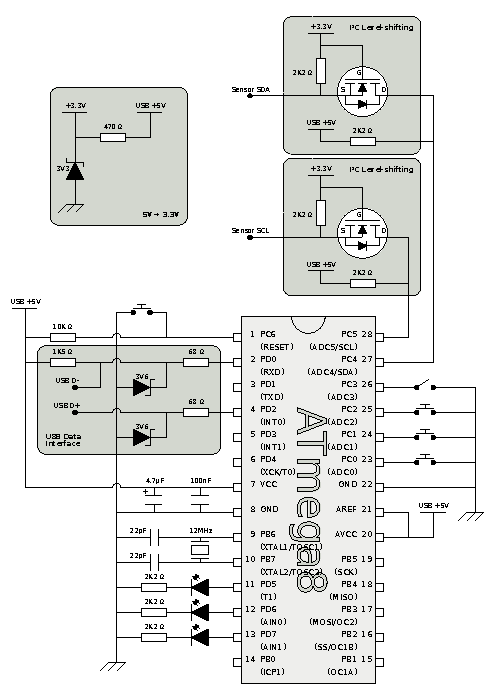
\includegraphics[keepaspectratio, width=1.0\textwidth, height=0.8\textheight, clip, viewport=1.33in 2.66in 3.00in 3.66in]{../monografia/img/AVR-magnetometer-usb-mouse.pdf}
	\end{center}
\end{frame}


\begin{frame}{I²C Level-shifting}
	\begin{center}
		% viewport parameter order: left bottom left+width bottom+height
		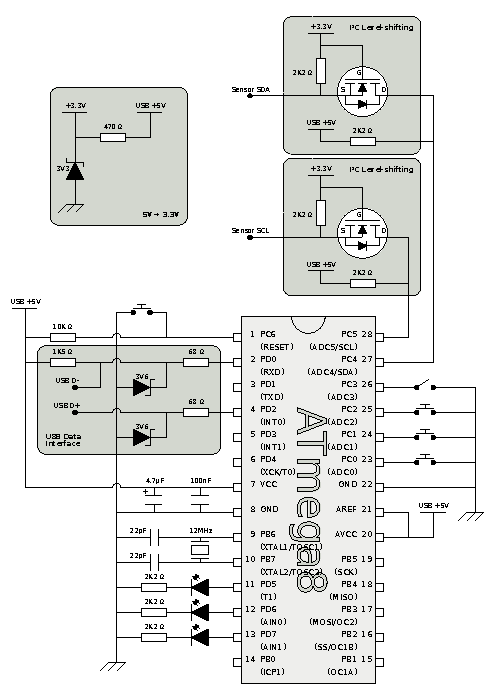
\includegraphics[keepaspectratio, width=1.0\textwidth, height=0.8\textheight, clip, viewport=1.33in 3.56in 3.00in 4.56in]{../monografia/img/AVR-magnetometer-usb-mouse.pdf}
	\end{center}
\end{frame}


\subsection{LEDs e botões}

\againframe[plain]{circuito-portrait}

\againframe[plain]{circuito-landscape}


\begin{frame}{LEDs e botões}
	\begin{columns}
		\column{.5\textwidth}
		\begin{center}
			% viewport parameter order: left bottom left+width bottom+height
			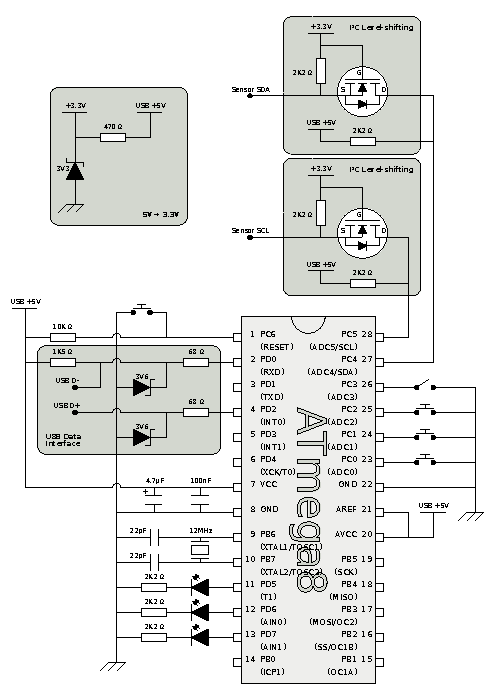
\includegraphics[keepaspectratio, width=1.0\textwidth, height=0.8\textheight, clip, viewport=0.66in 0.10in 2.00in 1.66in]{../monografia/img/AVR-magnetometer-usb-mouse.pdf}
		\end{center}

		\column{.5\textwidth}
		\begin{center}
			% viewport parameter order: left bottom left+width bottom+height
			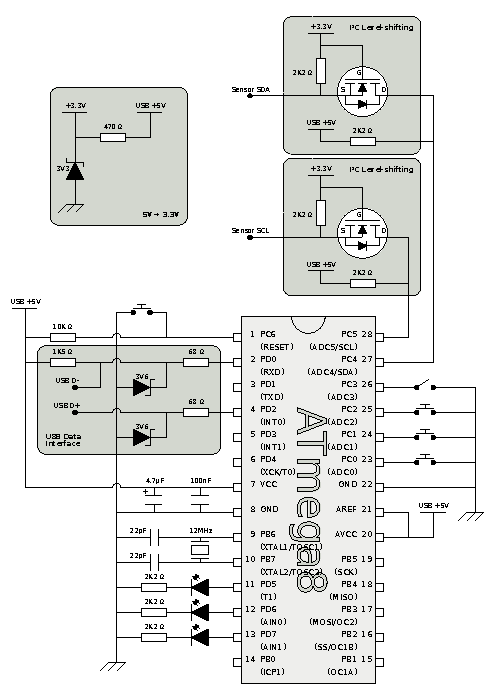
\includegraphics[keepaspectratio, width=1.0\textwidth, height=0.8\textheight, clip, viewport=2.00in 1.00in 3.33in 2.56in]{../monografia/img/AVR-magnetometer-usb-mouse.pdf}
		\end{center}
	\end{columns}
\end{frame}


\section{Software}

\subsection{Ambiente de desenvolvimento}

\begin{frame}{Ambiente de desenvolvimento (software)}
	\begin{itemize}
		\pause
		\item AVR-GCC 4.5.3, AVR-Libc 1.7.0
		\pause
		\item AVRDUDE 5.5
		\pause
		\item Software livre e multi-plataforma
		\pause
		\item Disponível para FreeBSD, Linux, Mac OS X \pause e Windows
	\end{itemize}
\end{frame}


\begin{frame}{Ambiente de desenvolvimento (hardware)}
	\pause
	USBasp
	\begin{itemize}
		\pause
		\item Gravador de microcontroladores AVR
		\pause
		\item ISP -- In-System Programming
		\pause
		\item Interface USB
		\pause
		\item Construído usando um microcontrolador AVR
		\pause
		\item Software livre
		\pause
		\item Comprado no eBay por apenas 6 dólares
	\end{itemize}
\end{frame}


\begin{frame}{USBasp}
	\begin{center}
		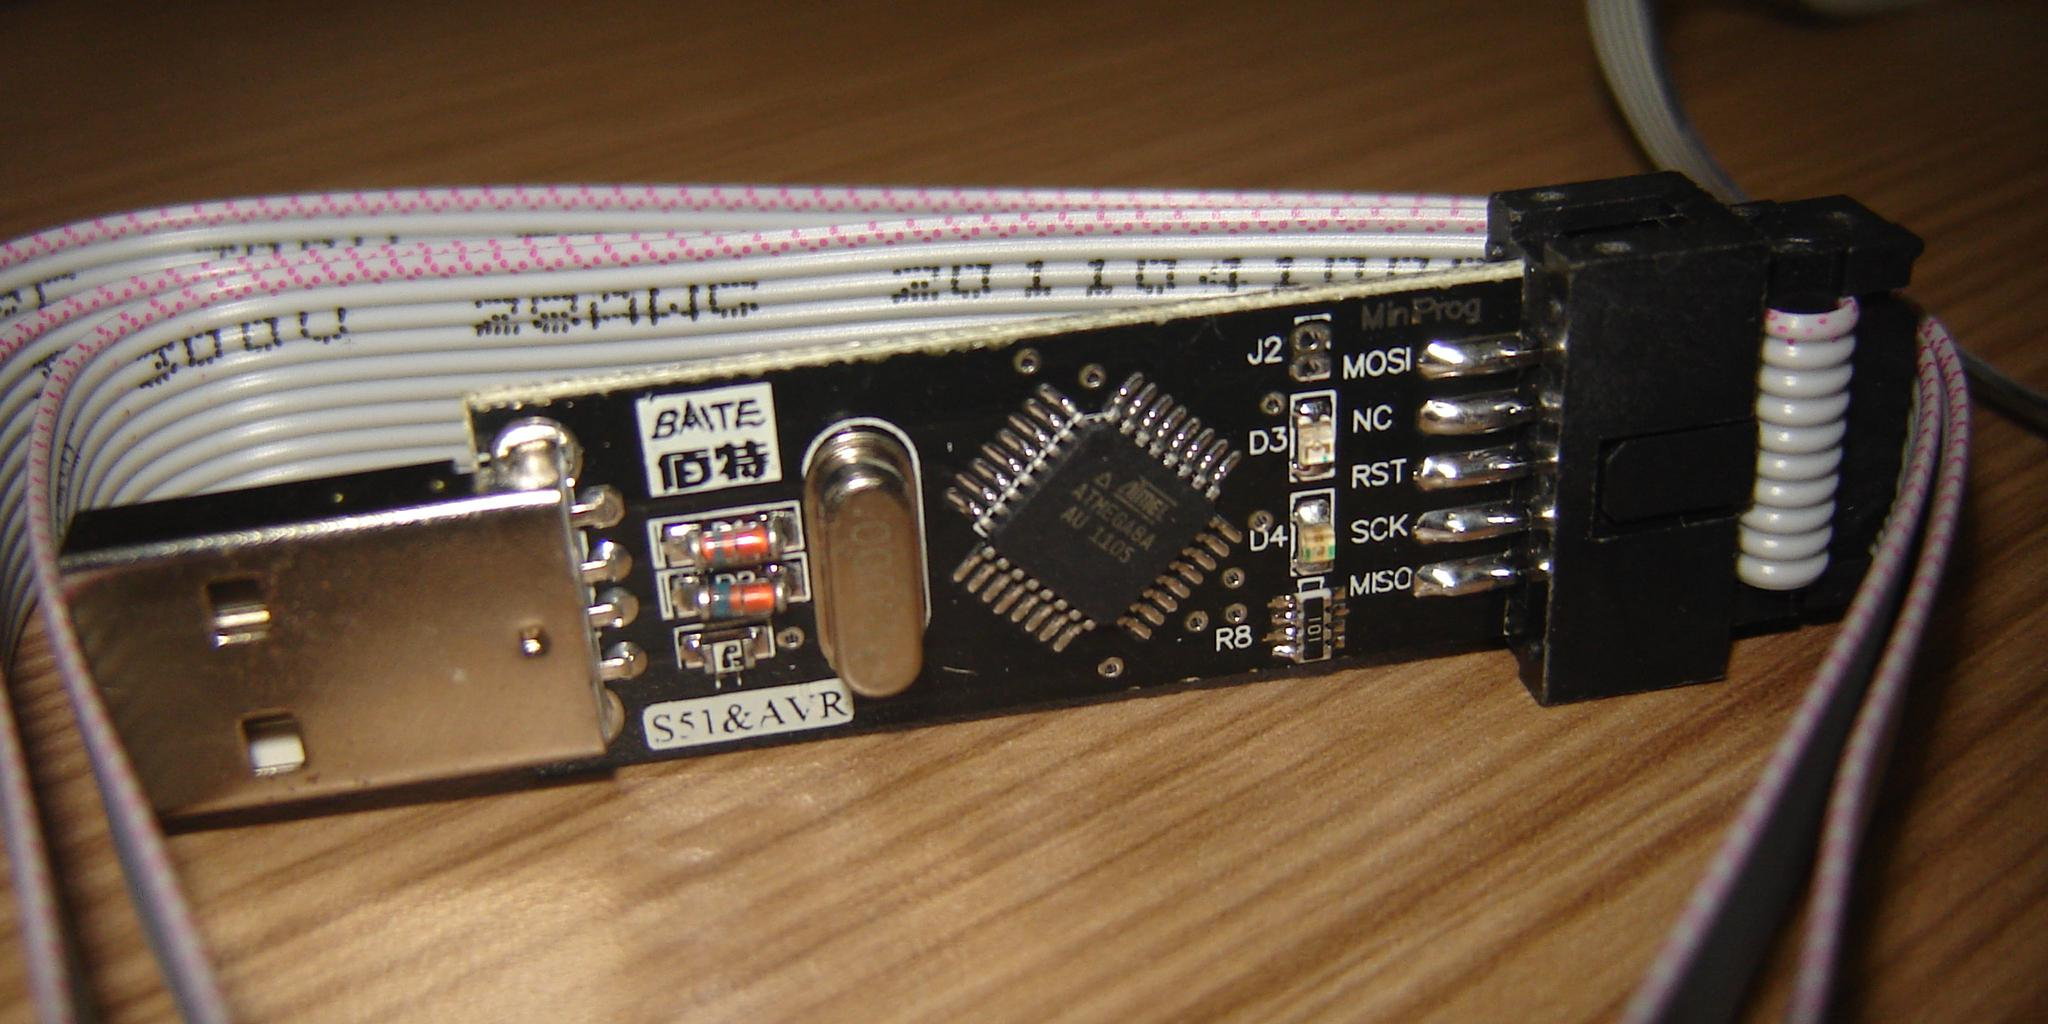
\includegraphics[height=0.4\textheight]{img/usbasp_top_hi.jpg}

		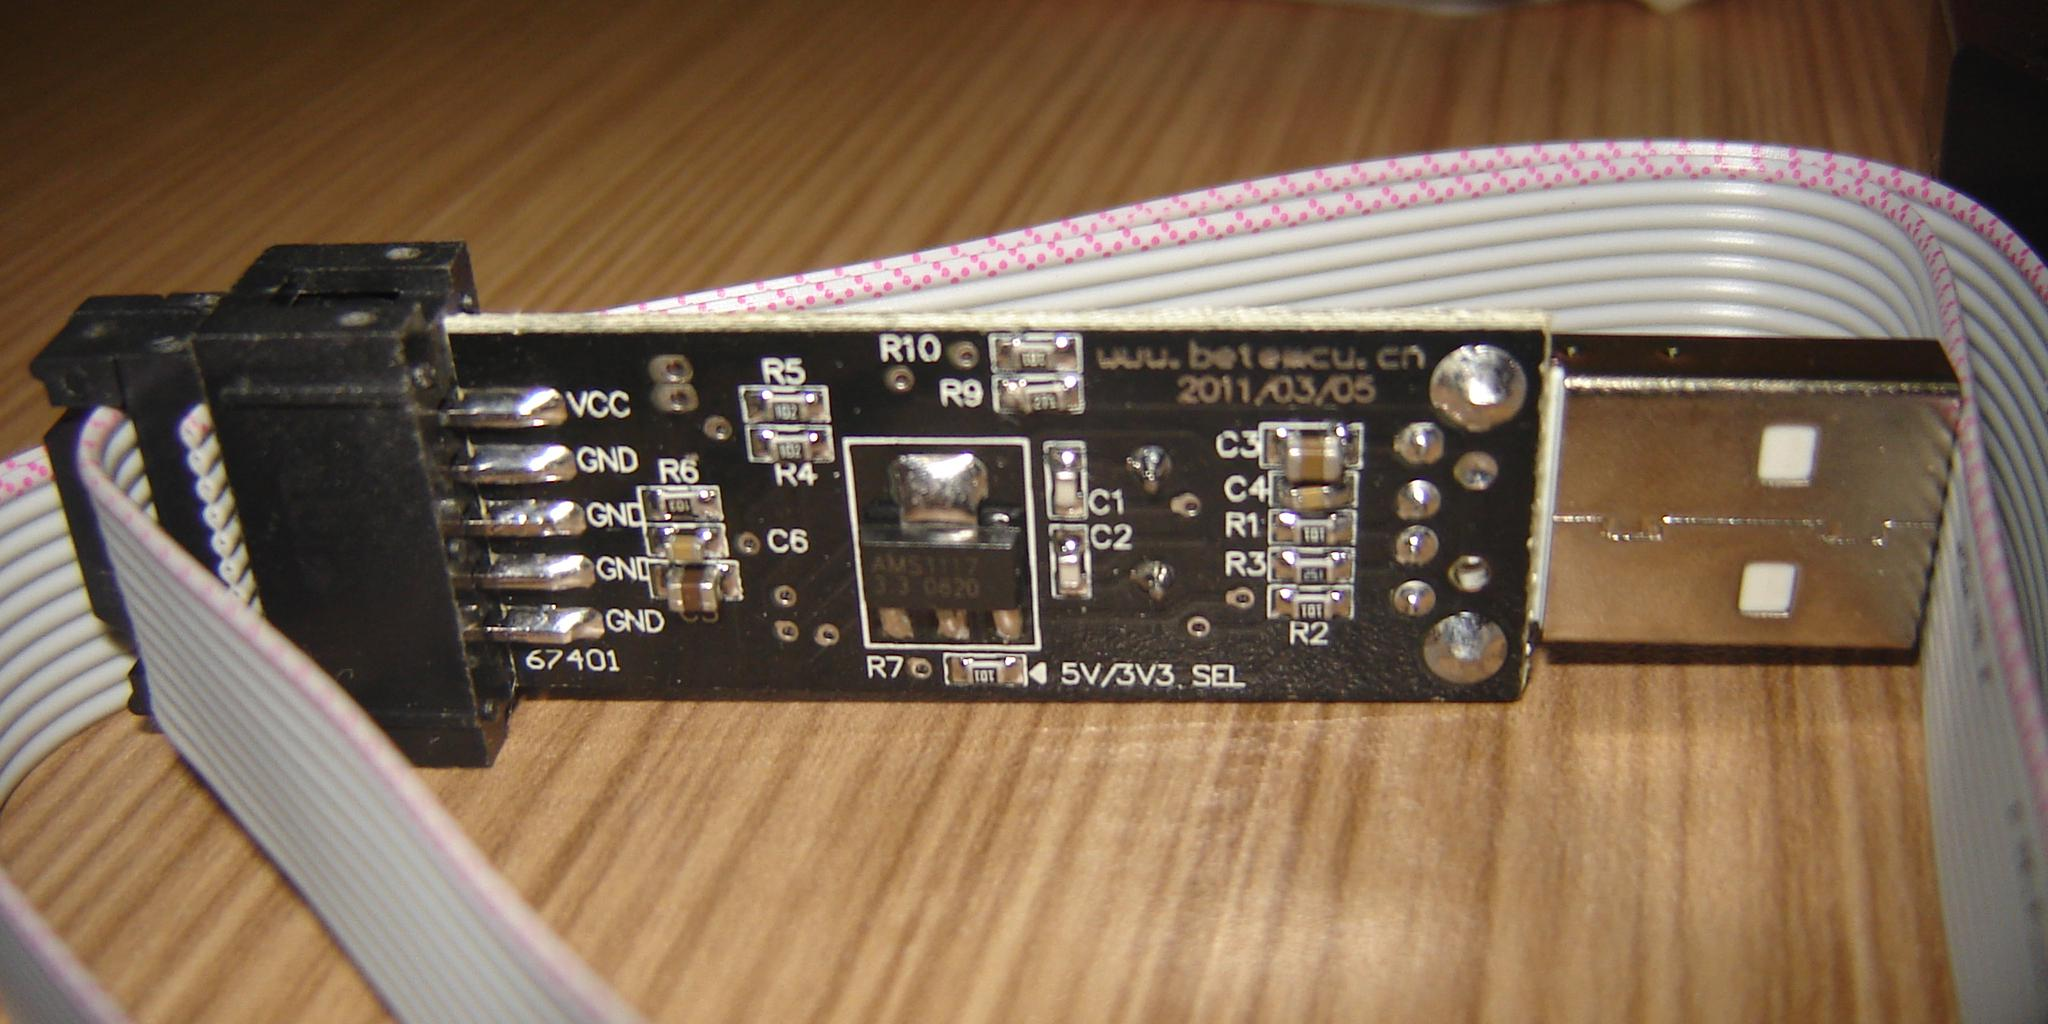
\includegraphics[height=0.4\textheight]{img/usbasp_bottom_hi.jpg}
	\end{center}
\end{frame}


\begin{frame}[plain]
	\begin{center}
		% trim parameter order: left bottom right top
		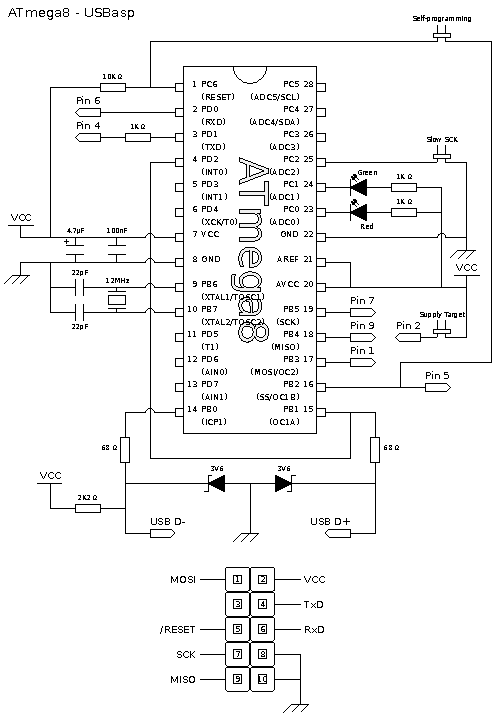
\includegraphics[keepaspectratio, width=1.0\textwidth, height=1.0\textheight, clip, trim=0.00in 1.10in 0.00in 0.00in]{img/AVR-USBasp.pdf}
	\end{center}
\end{frame}


\begin{frame}{USBasp}
	\begin{center}
		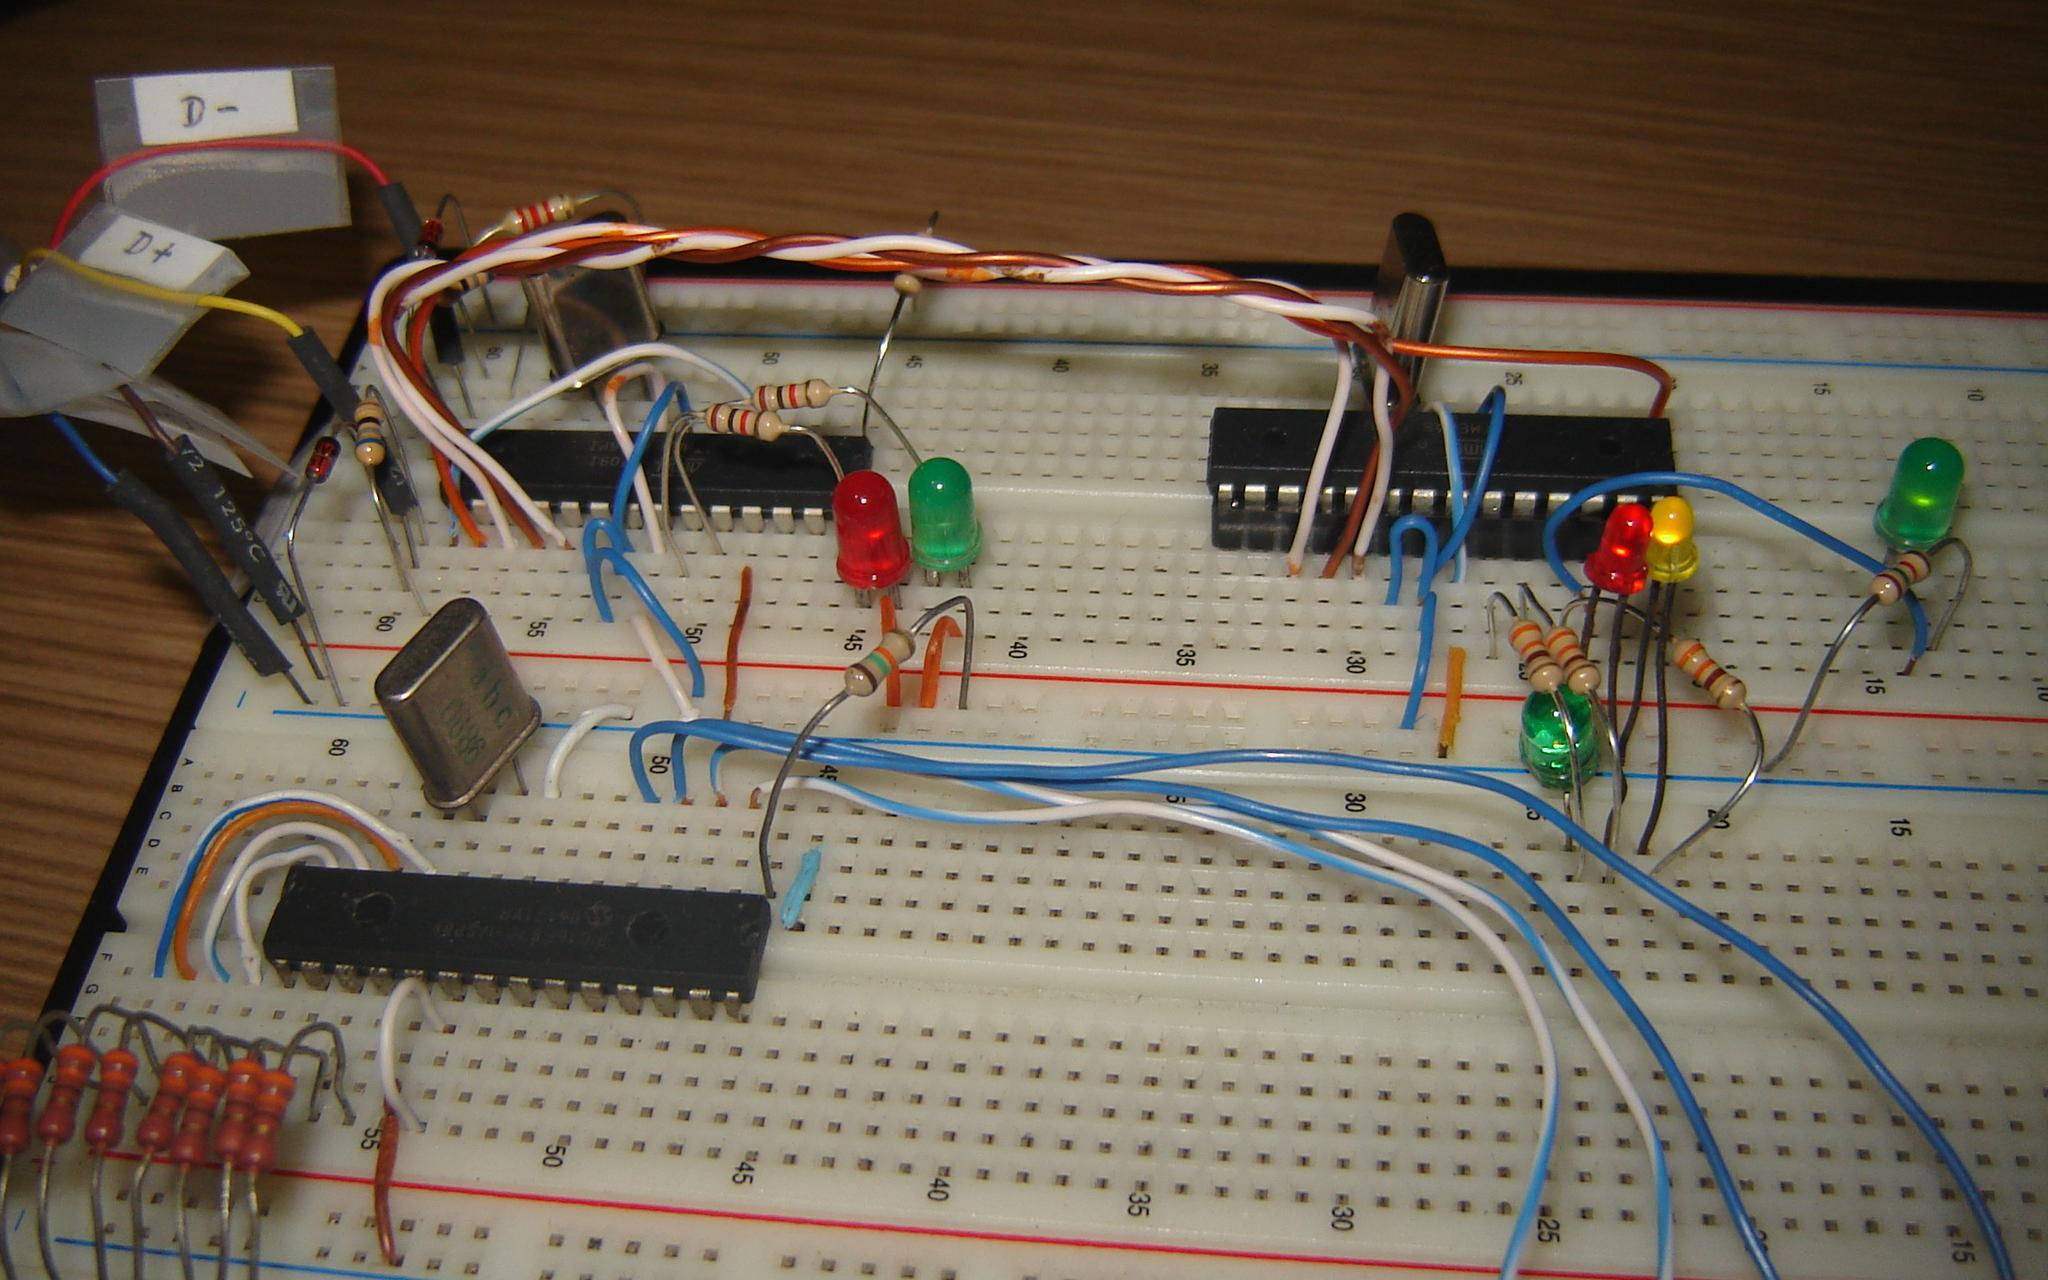
\includegraphics[keepaspectratio, width=1.0\textwidth, height=0.8\textheight, clip, trim=0.00in 5.75in 0.00in 0.00in]{img/usbasp_on_breadboard_2_hi.jpg}
	\end{center}
\end{frame}


\subsection{Visão geral}

\begin{frame}{Visão geral do firmware}
	\begin{itemize}
		\pause
		\item Comunicação I²C com o sensor
		\pause
		\item Comunicação USB com o computador
		\begin{itemize}
			\pause
			\item Teclado\pause, usado para implementar um menu de configuração
			\pause
			\item Mouse\pause, que na verdade é um \emph{absolute pointing device}
		\end{itemize}
		\pause
		\item Transformação de coordenadas
	\end{itemize}
\end{frame}


\subsection{Comunicação I²C com o sensor}

\begin{frame}{Comunicação I²C com o sensor}
	\pause
	\begin{itemize}[<+->]
		\item AVR315: Using the TWI module as I²C master
		\item Baseada em interrupção
	\end{itemize}
\end{frame}


\begin{frame}{Configuração do sensor}
	\begin{itemize}
		\pause
		\item Medições a \SI{75}{\hertz}
		\pause
		\item Cada medição é uma média de 8 leituras
		\pause
		\item Ganho de ±\SI{1.3}{\gauss}
		\pause
		\begin{itemize}
			\item \num{1090} bits por gauss
			\item \SI{0.92}{\milli\gauss} por bit
			\pause
			\item Escolhido por obter o máximo de precisão sem causar overflow
		\end{itemize}
		\pause
		\item Polling para receber as medições do sensor
		\begin{itemize}
			\pause
			\item \SI{146}{\hertz} através do Timer0 do microcontrolador
			\pause
			\item Pino DRDY permitiria uma abordagem por interrupção
		\end{itemize}
	\end{itemize}
\end{frame}

\againframe{fotos-sensor}


\subsection{Comunicação USB}

\begin{frame}{Comunicação USB}
	\begin{itemize}
		\pause
		\item ATmega8 não possui hardware dedicado para USB
		\pause
		\item Driver V-USB
		\begin{itemize}
			\item Suporte a USB implementado por software
			\pause
			\item Desenvolvido pela Objective Development Software GmbH.
			\pause
			\item Usado por mais de 100 projetos\pause, inclusive o USBasp
		\end{itemize}
	\end{itemize}
\end{frame}


\begin{frame}{Teclado USB}
	\begin{itemize}
		\pause
		\item Não implementa o protocolo \emph{boot}
		\pause
		\item \emph{Report} de 3 bytes:
		\begin{itemize}
			\pause
			\item \emph{Report ID} com valor 1
			\pause
			\item 8 bits para as teclas modificadoras
			\begin{itemize}
				\pause
				\item Apenas a tecla \emph{left shift} é usada
			\end{itemize}
			\pause
			\item 1 byte para a tecla sendo pressionada
		\end{itemize}
	\end{itemize}
\end{frame}


\begin{frame}[fragile]{USB Report Descriptor para o teclado}
	\begin{ccodesmall}
	0x05, 0x01,        // USAGE_PAGE (Generic Desktop)
	0x09, 0x06,        // USAGE (Keyboard)
	0xa1, 0x01,        // COLLECTION (Application)
	0x85, 0x01,	       //   REPORT_ID (1)
	// Modifier keys
	0x05, 0x07,        //   USAGE_PAGE (Keyboard)
	0x19, 0xe0,        //   USAGE_MINIMUM (Keyboard LeftControl)
	0x29, 0xe7,        //   USAGE_MAXIMUM (Keyboard Right GUI)
	0x15, 0x00,        //   LOGICAL_MINIMUM (0)
	0x25, 0x01,        //   LOGICAL_MAXIMUM (1)
	0x75, 0x01,        //   REPORT_SIZE (1)
	0x95, 0x08,        //   REPORT_COUNT (8)
	0x81, 0x02,        //   INPUT (Data,Var,Abs)
	// Normal keys
	0x05, 0x07,        //   USAGE_PAGE (Keyboard)
	0x19, 0x00,        //   USAGE_MINIMUM (Reserved (no event indicated))
	0x29, 0x65,        //   USAGE_MAXIMUM (Keyboard Application)
	0x15, 0x00,        //   LOGICAL_MINIMUM (0)
	0x25, 0x65,        //   LOGICAL_MAXIMUM (101)
	0x75, 0x08,        //   REPORT_SIZE (8)
	0x95, 0x01,        //   REPORT_COUNT (1)
	0x81, 0x00,        //   INPUT (Data,Ary,Abs)
	0xc0,              // END_COLLECTION
	\end{ccodesmall}
\end{frame}


\begin{frame}{Mouse USB}
	\begin{itemize}
		\pause
		\item Não implementa o protocolo \emph{boot}
		\pause
		\item \emph{Report} de 6 bytes:
		\begin{itemize}
			\pause
			\item \emph{Report ID} com valor 2
			\pause
			\item 2 bytes para a coordenada X
			\item 2 bytes para a coordenada Y
			\begin{description}[Coordenadas absolutas]
				\pause
				\item[Coordenadas absolutas] \emph{absolute pointing device}
				\item[Coordenadas relativas] \emph{mouse} convencional
			\end{description}
			\pause
			\item 1 byte para os botões sendo pressionados
		\end{itemize}
	\end{itemize}
\end{frame}


\begin{frame}[fragile]{USB Report Descriptor para o mouse}
	\begin{ccodesmall}
	0x05, 0x01,        // USAGE_PAGE (Generic Desktop)
	0x09, 0x02,        // USAGE (Mouse)
	0xa1, 0x01,        // COLLECTION (Application)
	0x85, 0x02,	       //   REPORT_ID (2)
	0x09, 0x01,        //   USAGE (Pointer)
	0xa1, 0x00,        //   COLLECTION (Physical)
	// X, Y movement
	0x09, 0x30,        //     USAGE (X)
	0x09, 0x31,        //     USAGE (Y)
	0x15, 0x00,        //     LOGICAL_MINIMUM (0)
	0x26, 0xff, 0x7f,  //     LOGICAL_MAXIMUM (32767)
	0x75, 0x10,        //     REPORT_SIZE (16)
	0x95, 0x02,        //     REPORT_COUNT (2)
	0x81, 0x42,        //     INPUT (Data,Var,Abs,Null)
	0xc0,              //   END_COLLECTION
	// Buttons
	0x05, 0x09,        //   USAGE_PAGE (Button)
	0x19, 0x01,        //   USAGE_MINIMUM (Button 1)
	0x29, 0x03,        //   USAGE_MAXIMUM (Button 3)
	0x15, 0x00,        //   LOGICAL_MINIMUM (0)
	0x25, 0x01,        //   LOGICAL_MAXIMUM (1)
	0x75, 0x01,        //   REPORT_SIZE (1)
	0x95, 0x03,        //   REPORT_COUNT (3)
	0x81, 0x02,        //   INPUT (Data,Var,Abs)
	// Padding for the buttons
	0x75, 0x01,        //   REPORT_SIZE (1)
	0x95, 0x05,        //   REPORT_COUNT (5)
	0x81, 0x03,        //   INPUT (Cnst,Var,Abs)
	0xc0               // END_COLLECTION
	\end{ccodesmall}
\end{frame}


\begin{frame}[fragile]{Bug no kernel do Linux}
	\begin{itemize}
		\pause
		\item Segundo a especificação USB HID, valores fora dos limites lógicos de um campo devem ser ignorados
	\end{itemize}
	\pause
	\begin{ccode}[numbers=none]
	0x15, 0x00,        //     LOGICAL_MINIMUM (0)
	0x26, 0xff, 0x7f,  //     LOGICAL_MAXIMUM (32767)
	\end{ccode}
	\begin{itemize}
		\pause
		\item O bug foi reportado
		\pause
		\item Patch disponível
	\end{itemize}
	\begin{ccode}[numbers=none]
	if (value < field->logical_minimum ||
	    value > field->logical_maximum)
	{
	    dbg_hid("Ignoring out-of-range value %x\n", value);
	    return;
	}
	\end{ccode}
\end{frame}


\begin{frame}{Oscilação do ponteiro}
	Possíveis causas:
	\begin{itemize}
		\pause
		\item Limite de precisão do sensor
		\pause
		\item Limite de precisão do conversor ADC
		\pause
		\item Interferência magnética de aparelhos elétricos e eletrônicos
	\end{itemize}
\end{frame}


\begin{frame}{Suavização do movimento}
	\pause
	Filtro de suavização exponencial:
	\pause
	\begin{align*}
		x_t & = 0.875 x_{t-1} + 0.125 x
	\end{align*}
	\begin{itemize}
		\pause
		\item Introduz um pequeno atraso no movimento
		\pause
		\item Aumenta notavelmente a precisão
	\end{itemize}
	\pause
	\bigskip
	Além disso:
	\begin{itemize}
		\pause
		\item Movimento do ponteiro é congelado por \SI{87}{\milli\second} após um clique
	\end{itemize}
\end{frame}


\begin{frame}{Menu de configuração}
	\begin{itemize}
		\pause
		\item Implementado usando o teclado USB
		\pause
		\item Usável dentro de qualquer editor de texto
		\pause
		\item Simplifica a configuração e depuração do dispositivo
	\end{itemize}
\end{frame}


\section{Matemática}

\subsection{Introdução}

\begin{frame}{Definição do problema}
	\pause
	Dado um vetor 3D apontando para uma direção qualquer no espaço,
	quais são as coordenadas 2D correspondentes a esse vetor?
	\pause
	\bigskip
	\begin{center}
	% trim parameter order: left bottom right top
	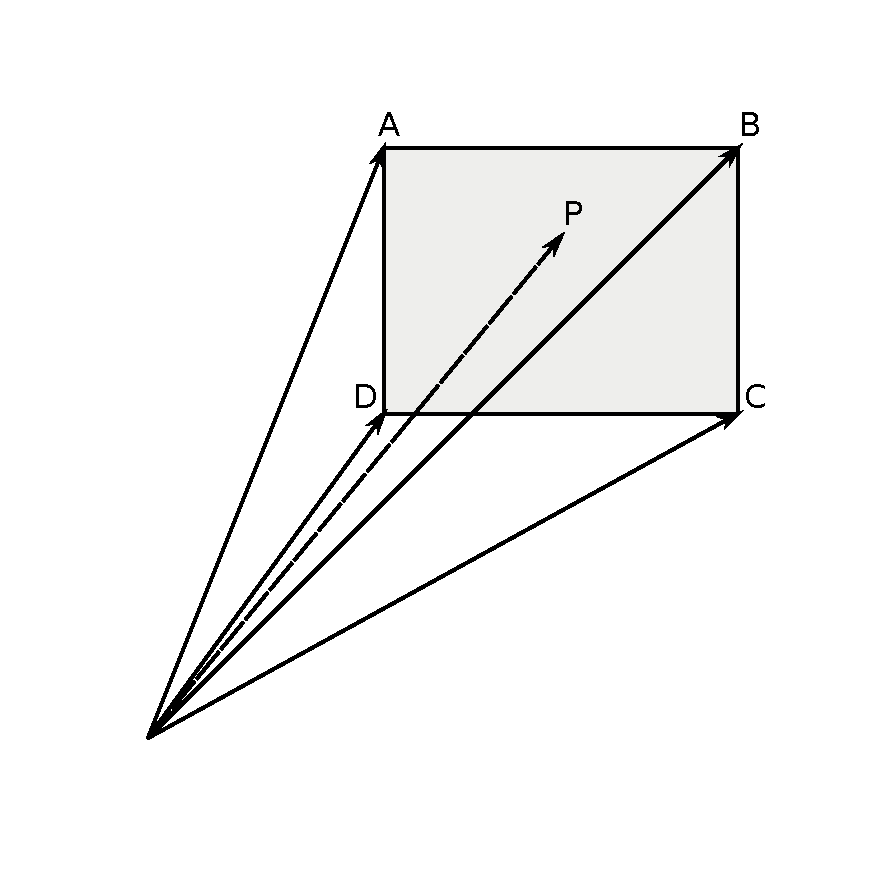
\includegraphics[keepaspectratio, width=1.0\textwidth, height=0.5\textheight, clip, trim=0.75in 0.75in 0.70in 0.50in]{../monografia/img/geometria_ABCD1.pdf}
	\end{center}
\end{frame}


\subsection{Abordagem geométrica}

\begin{frame}{Abordagem geométrica}
	\begin{center}
	% trim parameter order: left bottom right top
	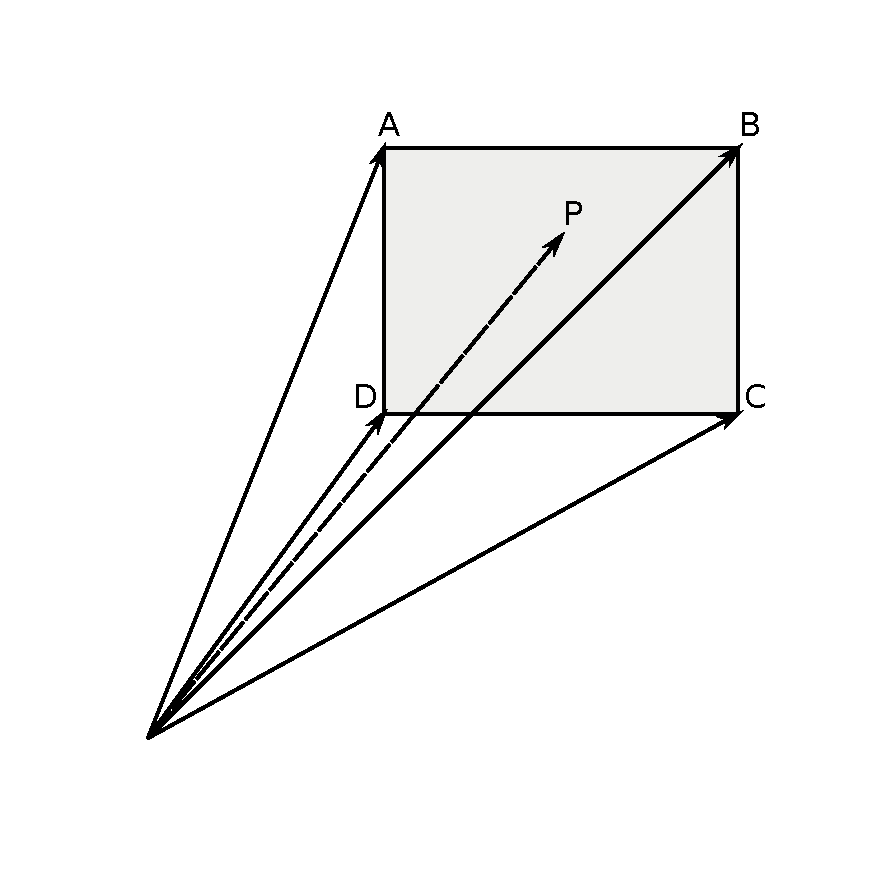
\includegraphics[keepaspectratio, width=1.0\textwidth, height=0.8\textheight, clip, trim=0.75in 0.75in 0.70in 0.50in]{../monografia/img/geometria_ABCD1.pdf}
	\end{center}
\end{frame}

\begin{frame}{Abordagem geométrica}
	\begin{center}
	% trim parameter order: left bottom right top
	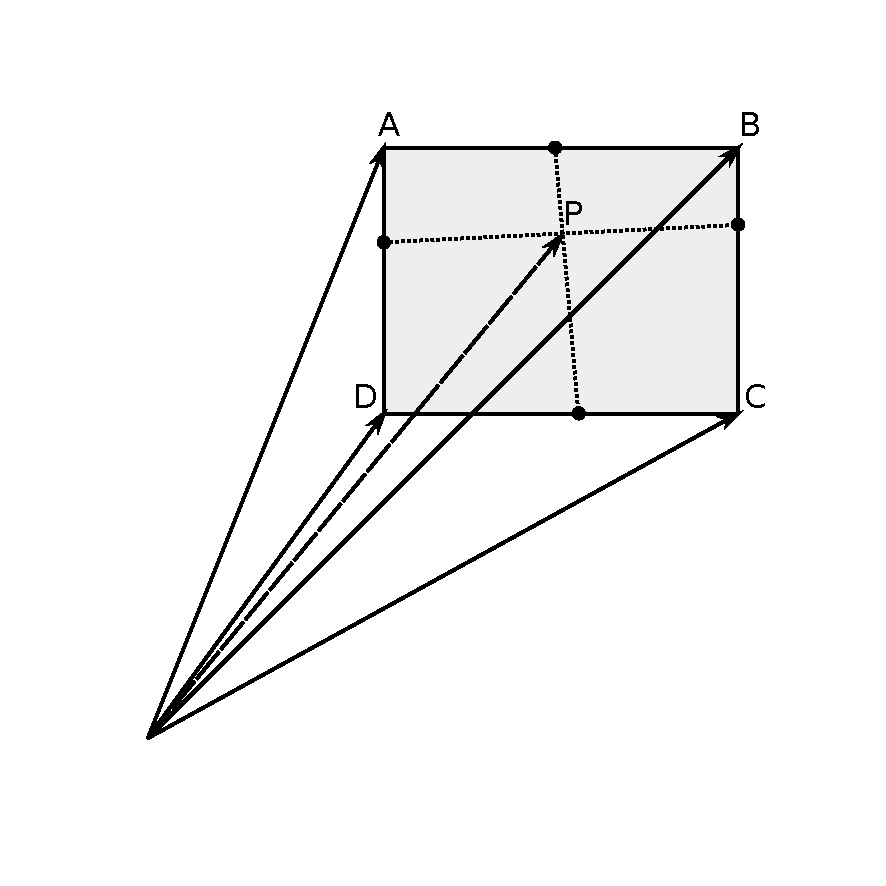
\includegraphics[keepaspectratio, width=1.0\textwidth, height=0.8\textheight, clip, trim=0.75in 0.75in 0.70in 0.50in]{../monografia/img/geometria_ABCD2.pdf}
	\end{center}
\end{frame}


\begin{frame}{Abordagem geométrica -- definições}
	\begin{columns}
		\column{.5\textwidth}
		\pause
		Sejam os vetores:
		\begin{description}[A]
		\item[A] Aponta na direção do canto superior esquerdo da tela
		\item[B] Aponta na direção do canto superior direito da tela
		\item[C] Aponta na direção do canto inferior direito da tela
		\item[D] Aponta na direção do canto inferior esquerdo da tela
		\item[P] Direção apontada pelo usuário
		\end{description}
		Todos com origem em $(0,0,0)$

		\column{.5\textwidth}
		\onslide<1->
		% trim parameter order: left bottom right top
		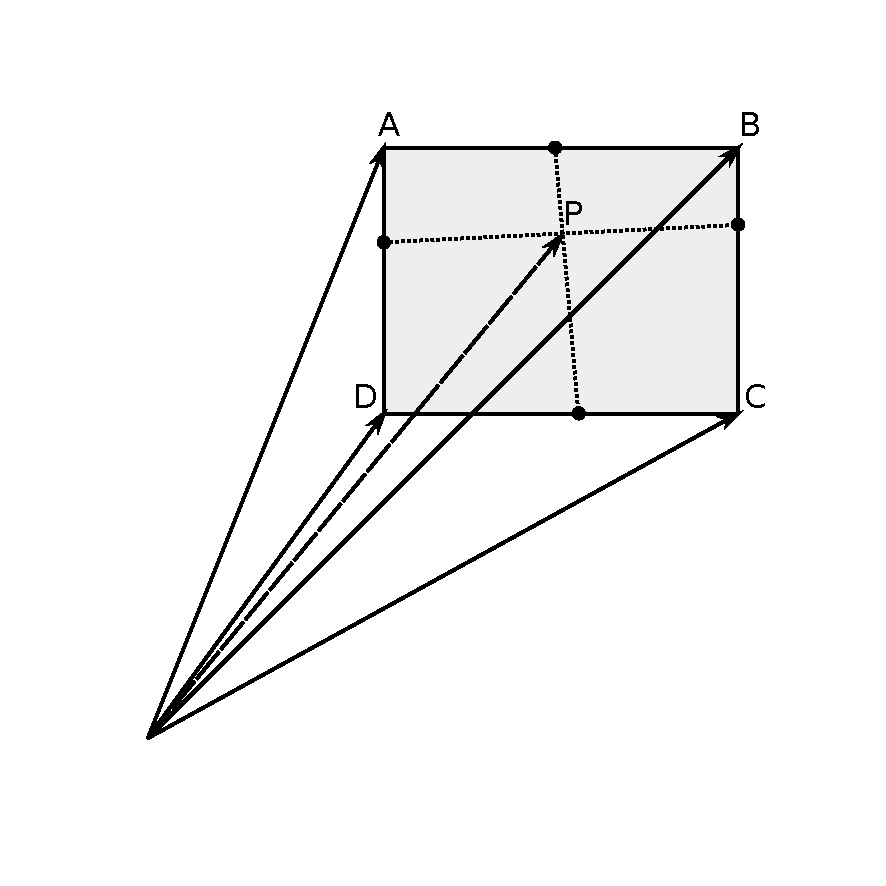
\includegraphics[keepaspectratio, width=1.0\textwidth, height=0.8\textheight, clip, trim=0.75in 0.75in 0.70in 0.50in]{../monografia/img/geometria_ABCD2.pdf}
	\end{columns}
\end{frame}


\begin{frame}{Abordagem geométrica -- algoritmo}
	\begin{columns}
		\column{.5\textwidth}
		\begin{enumerate}[<+->]
		\item Calcular $P'$, projeção de $P$ no plano definido por $A$ e $B$
		\item Calcular $\alpha$, valor entre $0$ e $1$ tal que:
			\begin{itemize}
			\item $\alpha = 0 \iff P' \parallel A $
			\item $\alpha = 1 \iff P' \parallel B $
			\end{itemize}
		\item Repetir os cálculos para cada um dos quatro lados
		\item Usar os quatro valores de $\alpha$ para estimar as coordenadas 2D no plano da tela
		\end{enumerate}

		\column{.5\textwidth}
		\onslide<1->
		% trim parameter order: left bottom right top
		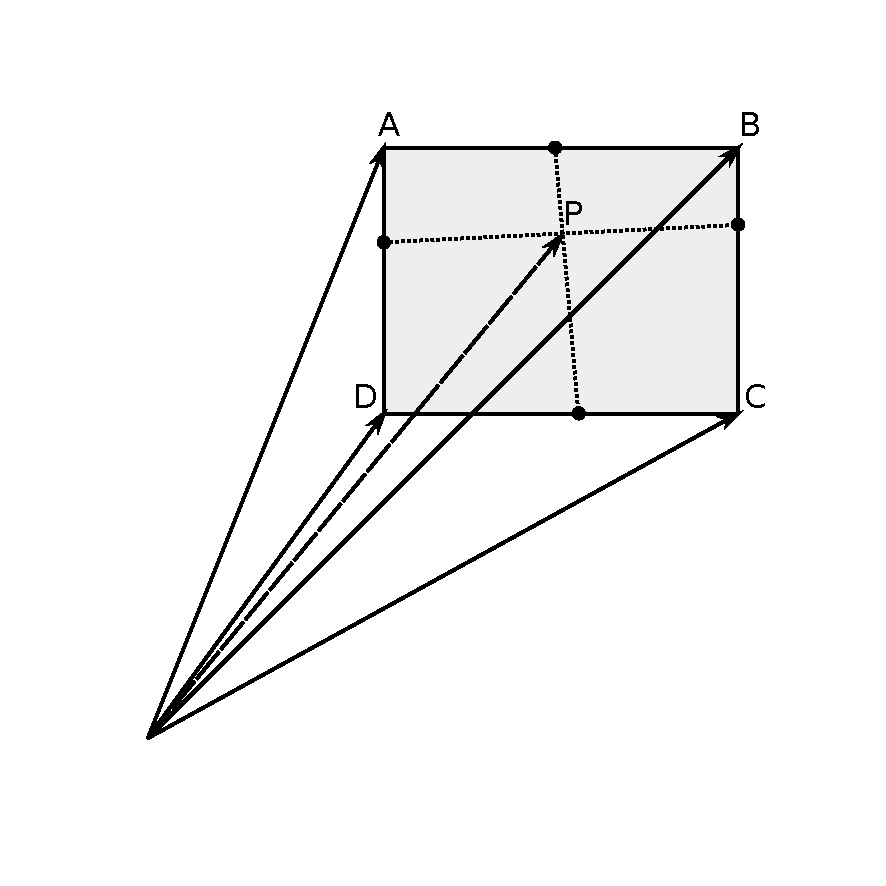
\includegraphics[keepaspectratio, width=1.0\textwidth, height=0.8\textheight, clip, trim=0.75in 0.75in 0.70in 0.50in]{../monografia/img/geometria_ABCD2.pdf}
	\end{columns}
\end{frame}


\begin{frame}{Abordagem geométrica -- cálculo de $\alpha$}
	\begin{columns}
		\column{.5\textwidth}
		Como calcular $\alpha$?
		\begin{itemize}
		\pause
		\item Valor exato, interseção de $P'$ com o segmento $AB$
		\pause
		\item Valor aproximado...
		\end{itemize}

		\column{.5\textwidth}
		\onslide<1->
		% trim parameter order: left bottom right top
		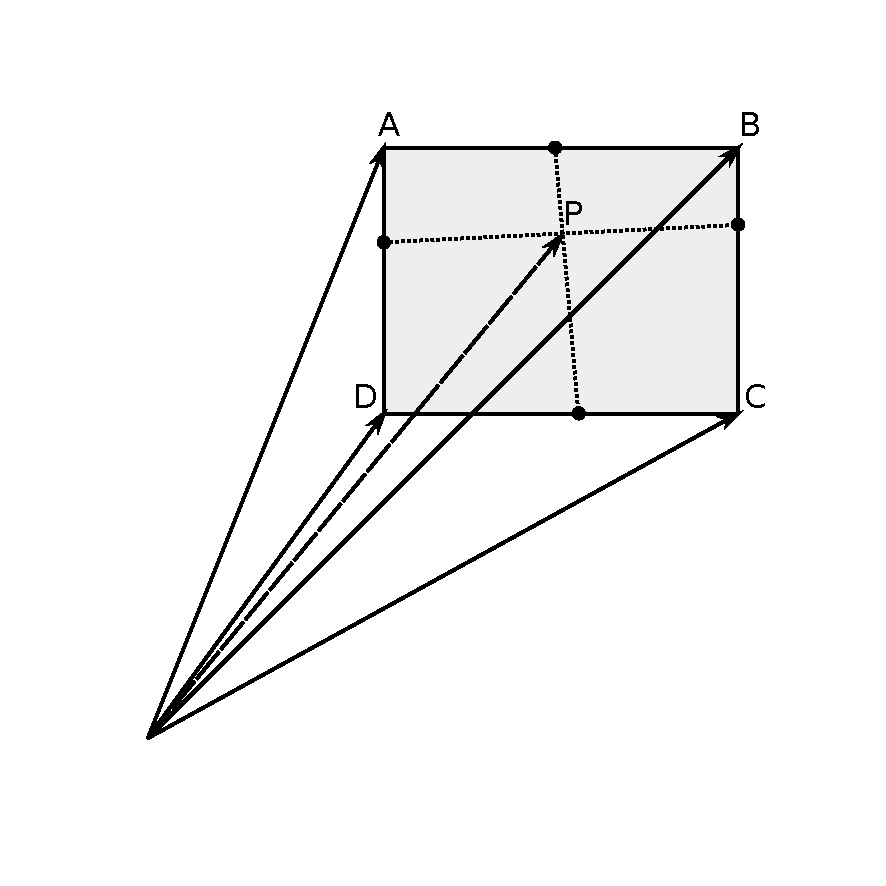
\includegraphics[keepaspectratio, width=1.0\textwidth, height=0.8\textheight, clip, trim=0.75in 0.75in 0.70in 0.50in]{../monografia/img/geometria_ABCD2.pdf}
	\end{columns}
\end{frame}


\begin{frame}{Abordagem geométrica -- cálculo de $\alpha$}
	\begin{columns}
		\column{.5\textwidth}
		\begin{align*}
		\alpha & = \frac{\angulo(A, P')}{\angulo(A, B)} \\
		\alpha & = \frac{
				\left| \dfrac{A}{|A|} - \dfrac{P'}{|P'|} \right|
			}{
				\left| \dfrac{A}{|A|} - \dfrac{B }{|B |} \right|
			}  \\
		\alpha & = \frac{\sin(\angulo(A, P'))}{\sin(\angulo(A, B))} \\
		\alpha & = \frac{\cos(\angulo(A, P'))}{\cos(\angulo(A, B))} \\
		\alpha & = \frac{\tan(\angulo(A, P'))}{\tan(\angulo(A, B))}
		\end{align*}

		\column{.5\textwidth}
		\onslide<1->
		% trim parameter order: left bottom right top
		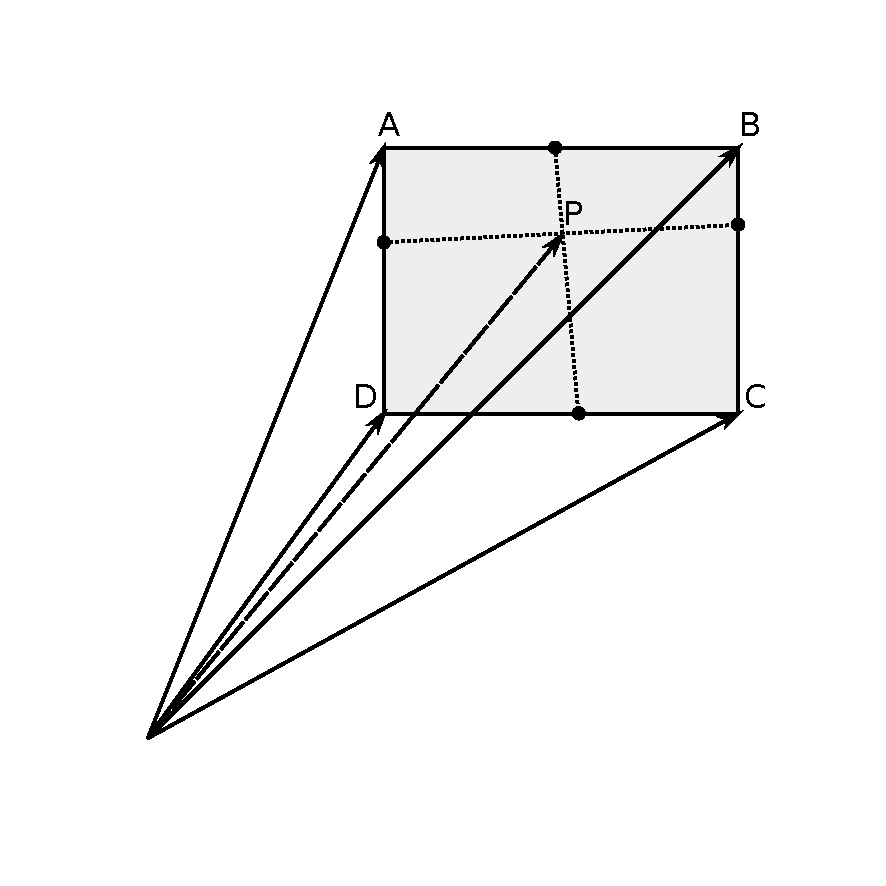
\includegraphics[keepaspectratio, width=1.0\textwidth, height=0.8\textheight, clip, trim=0.75in 0.75in 0.70in 0.50in]{../monografia/img/geometria_ABCD2.pdf}
	\end{columns}
\end{frame}


\subsection{Abordagem por sistema linear}

\begin{frame}{Abordagem por sistema linear -- definições}
	\begin{columns}
		\column{.5\textwidth}
		\pause
		Sejam os vetores:
		\begin{description}[A]
		\item[A] Aponta na direção do canto superior esquerdo da tela
		\item[B] Aponta na direção do canto superior direito da tela
		\item[D] Aponta na direção do canto inferior esquerdo da tela
		\item[P] Direção apontada pelo usuário
		\end{description}
		Todos com origem em $(0,0,0)$

		\column{.5\textwidth}
		\onslide<1->
		% trim parameter order: left bottom right top
		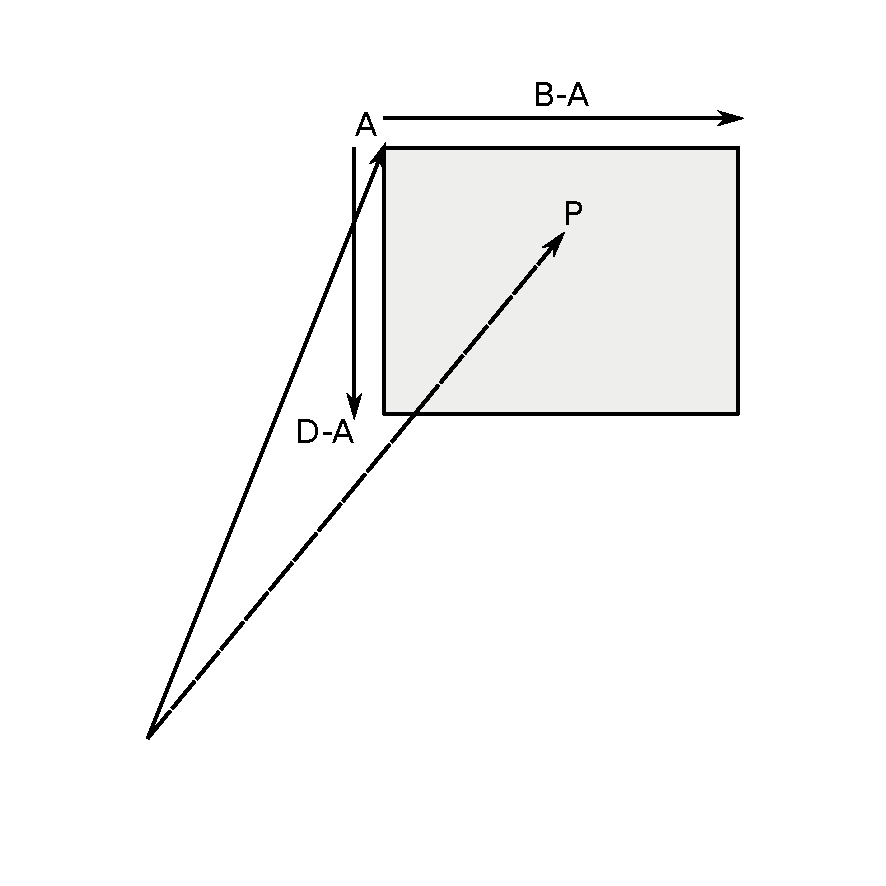
\includegraphics[keepaspectratio, width=1.0\textwidth, height=0.8\textheight, clip, trim=0.75in 0.75in 0.70in 0.50in]{../monografia/img/lineq.pdf}
	\end{columns}
\end{frame}

\begin{frame}{Abordagem por sistema linear}
	\begin{columns}
		\column{.5\textwidth}
		\pause
		O vetor P pode ser escrito como:

		\begin{equation*}
		zP = A + x(B-A) + y(D-A)
		\end{equation*}

		\pause
		Que é equivalente à equação:

		\begin{equation*}
		x(B-A) + y(D-A) - zP = -A
		\end{equation*}

		\column{.5\textwidth}
		\onslide<1->
		% trim parameter order: left bottom right top
		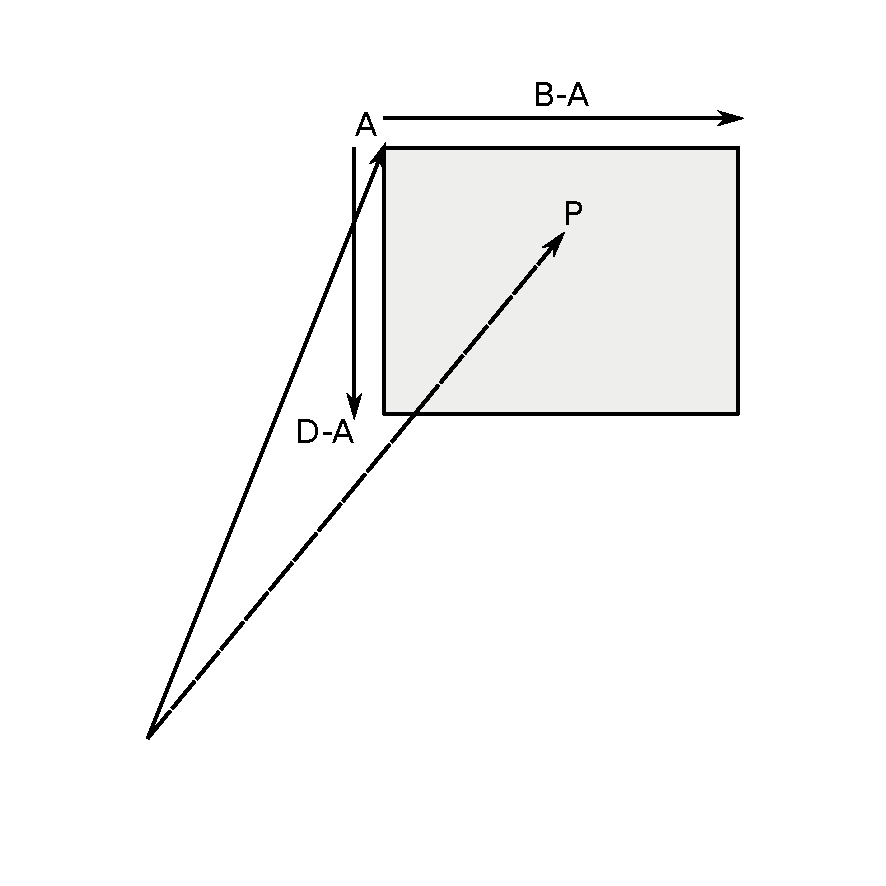
\includegraphics[keepaspectratio, width=1.0\textwidth, height=0.8\textheight, clip, trim=0.75in 0.75in 0.70in 0.50in]{../monografia/img/lineq.pdf}
	\end{columns}
\end{frame}


\subsection{Outras abordagens}

\begin{frame}{Outras abordagens}
	\pause
	\begin{itemize}
	\item Coordenadas esféricas $\phi$ e $\theta$
	\pause
	\item ...
	\end{itemize}
\end{frame}


\section{Conclusões}

\subsection{Resultados}

\begin{frame}{Resultados}
	\pause
	\begin{center}
	\Large{O dispositivo funciona!}
	\end{center}
	\pause
	Mas só funciona bem se a tela estiver virada para o Norte ou para o Sul.
\end{frame}

\begin{frame}[shrink=10]{Tamanho do firmware}
	\begin{columns}
		\column{.5\textwidth}
		\begin{center}
			\begin{tabular}{lr}
				\toprule

				\multicolumn{2}{c}{\texttt{make all}} \\

				\midrule

				\texttt{buttons}     &  138 bytes \\
				\texttt{int\_eeprom} &  156 bytes \\
				\texttt{TWI\_Master} &  351 bytes \\
				\texttt{keyemu}      &  372 bytes \\
				\texttt{main}        &  406 bytes \\
				\texttt{sensor}      &  446 bytes \\
				\texttt{usbdrvasm}   &  678 bytes \\
				\texttt{usbdrv}      &  792 bytes \\
				\texttt{mouseemu}    & 1492 bytes \\
				\texttt{menu}        & 1744 bytes \\

				%\midrule

				%Subtotal             & 6575 bytes \\
				AVR-Libc             & 1589 bytes \\

				\midrule

				Total                & 8164 bytes \\
				Livre                &   28 bytes \\

				\bottomrule
			\end{tabular}
		\end{center}

		\column{.5\textwidth}
		\begin{center}
			\begin{tabular}{lr}
				\toprule

				\multicolumn{2}{c}{\texttt{make combine}} \\

				\midrule

				Total                & 8040 bytes \\
				Livre                &  152 bytes \\

				\bottomrule
			\end{tabular}
		\end{center}
	\end{columns}
\end{frame}

\begin{frame}[plain]{}
	\begin{center}
		% trim parameter order: left bottom right top
		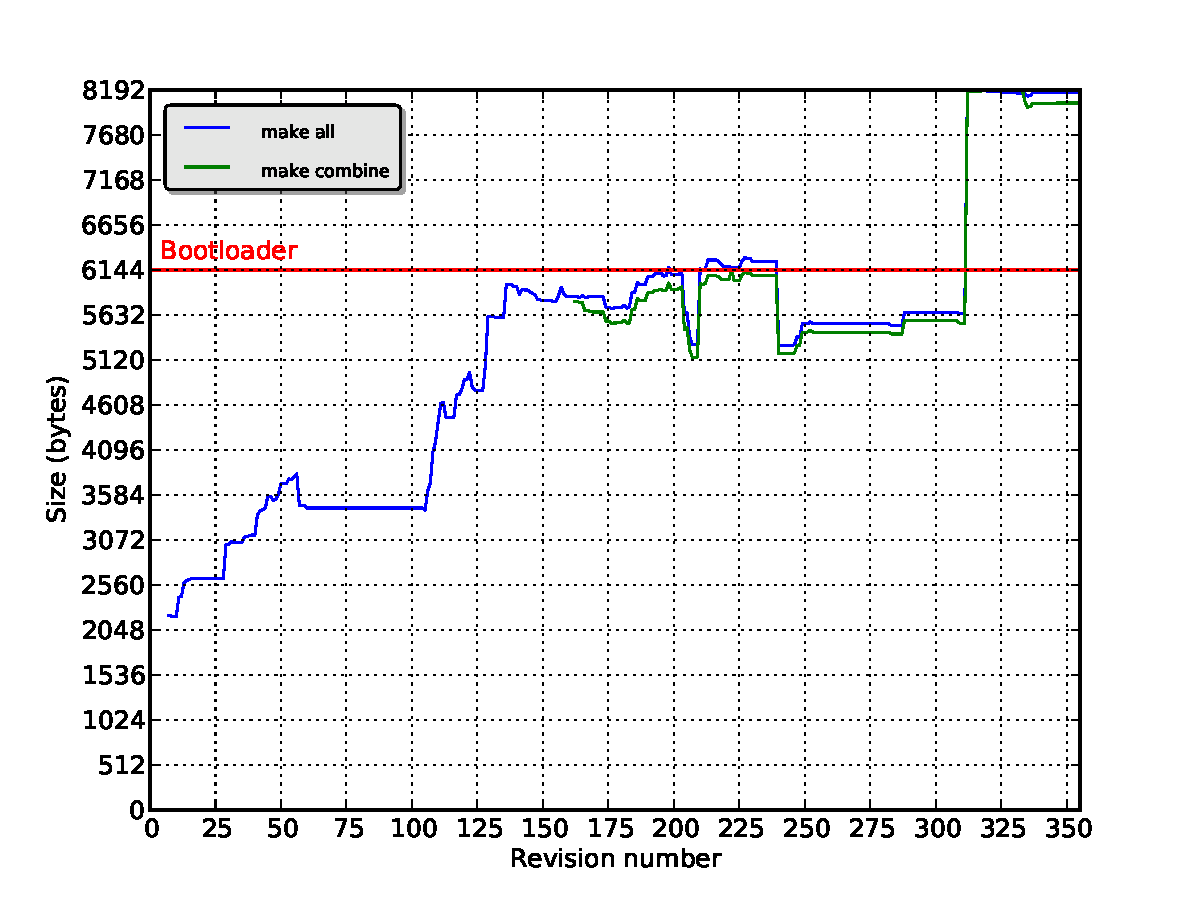
\includegraphics[keepaspectratio, width=1.0\textwidth, height=1.0\textheight, clip, trim=0.20in 0.20in 0.20in 0.20in]{img/firmware_size_graph.pdf}
	\end{center}
\end{frame}


\subsection{Trabalhos futuros}

\begin{frame}{Trabalhos futuros}
	\begin{itemize}
	\pause
	\item Usar dois sensores: magnetômetro e acelerômetro
		\begin{itemize}
		\pause
		\item Resolve a limitação de Norte-Sul
		\pause
		\item Magnetômetro $\Longrightarrow$ movimento horizontal
		\item Acelerômetro $\Longrightarrow$ movimento vertical
		\end{itemize}
	\pause
	\item Usar três sensores: magnetômetro, acelerômetro e giroscópio
		\begin{itemize}
		\pause
		\item Giroscópio aumentaria a precisão dos movimentos
		\end{itemize}
	\pause
	\item Implementar comunicação sem fio
	\end{itemize}
\end{frame}

\begin{frame}{Trabalhos futuros}
	\begin{itemize}
	\pause
	\item Produzir um produto para o mercado
		\begin{itemize}
		\pause
		\item Apontador para uso em apresentações e aulas
		\pause
		\item Dispositivo de acessibilidade para controlar o ponteiro com a cabeça ou outra parte do corpo
		\end{itemize}
	\end{itemize}
\end{frame}


\subsection{Fim}

\begin{frame}{}
	\begin{center}
	\Large{Obrigado!}
	\end{center}
\end{frame}


\end{document}
